\documentclass[12pt,a4paper]{report}
\usepackage{amsmath,amsthm,amssymb,graphicx,hyperref}
% \usepackage{lmodern}
% \usepackage{newtxtext,newtxmath}
\usepackage[left=1.2in,right=1in,top=1in,bottom=1in]{geometry}
\usepackage[romanian]{babel}
\usepackage{algorithm}
\usepackage{algpseudocode}
\usepackage{listings}
\usepackage[table]{xcolor}
\usepackage{xcolor}
\usepackage{subcaption}
\usepackage{tabularx}
\usepackage{multirow}
\usepackage{paralist}
\RequirePackage{hyphenat}
\usepackage{algorithm, algpseudocode}%algorithmic
\usepackage[inline]{enumitem}


%\usepackage{...insert other packages here...}
\newtheorem{thm}{Teorema}[section]
\newtheorem{lem}[thm]{Lema}
\newtheorem{cor}[thm]{Corolarul}
\newtheorem{prop}[thm]{Propozi\c tia}
\theoremstyle{definition}
\newtheorem{defn}{Defini\c tia}[section]
\theoremstyle{remark}
\newtheorem{rem}{Remarca}[section]
\newtheorem{exmp}{Exemplul}[section]

\def\contentsname{Cuprins}
\def\listfigurename{Lista figurilor}
\def\listtablename{Lista tabelelor}
\def\figurename{Figura}
\def\tablename{Tabelul}
\def\partname{Partea}
\def\chaptername{Capitolul}
\def\refname{Referin'te}
\def\bibname{Bibliografie} 
\def\appendixname{Anexa}

\begin{document}
\thispagestyle{empty}
\begin{center}
\begin{figure}[h!]
\vspace{-20pt}
\begin{center}

\includegraphics[width=100pt]{figs/FI.png}
\end{center}
\end{figure}


{\large{\bf UNIVERSITATEA DE VEST DIN TIMIȘOARA

FACULTATEA DE INFORMATICĂ

PROGRAMUL DE STUDII DE MASTER: Bioinformatică }}

\vspace{120pt}
{\huge {\bf LUCRARE DE DIZERTA\c TIE}}

\vspace{150pt}
\end{center}

{\large\noindent{\bf COORDONATOR:\hfill ABSOLVENT:}

\noindent Prof. Dr. Habil. Zaharie Daniela \hfill Smarandache Grigorie-Theodor}

\large\noindent Prof. Dr. Habil. Pârvulescu Lucian


\vfill
\begin{center}
{\bf TIMI\c SOARA

2026}
\end{center}
\newpage
\thispagestyle{empty}
\begin{center}
{\large{\bf UNIVERSITATEA DE VEST DIN TIMI\c SOARA

FACULTATEA DE INFORMATIC\u A


PROGRAMUL DE STUDII DE MASTER: Bioinformatic\u a }}

\vspace{120pt}
{\huge {\bf Identificarea automată a speciilor de raci din genul Austropotamobius prin tehnici de deep learning pe bază de imagini}}

\vspace{150pt}
\end{center}

{\large\noindent{\bf COORDONATOR:\hfill ABSOLVENT:}

\noindent Prof. Dr. Habil. Zaharie Daniela \hfill Smarandache Grigorie-Theodor}

\large\noindent Prof. Dr. Habil. Pârvulescu Lucian

\vfill
\begin{center}
{\bf TIMI\c SOARA

2026}
\end{center}
\newpage
\normalsize{}



\section*{Abstract}

Correctly identifying freshwater crayfish species of the genus \textit{Austropotamobius} is an important problem both from a biological and a practical standpoint, given that the presence and distribution of these crustaceans provide valuable indicators of aquatic habitat conditions. The task is made considerably more difficult by the pronounced morphological similarity between the two species addressed in this work, \textit{Austropotamobius bihariensis} and \textit{Austropotamobius torrentium}, which share a smooth carapace, a discreet postorbital ridge without a spine, and a triangular-shaped rostrum, differing only in fine details such as the relative length of the antennal scale or the roughness of the chelae. Additional intraspecific colour variability, particularly pronounced in \textit{A. torrentium}, further reduces the reliability of colour as a discriminative trait and increases the importance of shape and texture-based features. Manual identification is consequently dependent on evaluator experience and on the clarity of the available morphological cues, motivating the development of an automated, objective, and reproducible alternative.

This work proposes a binary automatic classification solution for the two species based on field photographs, using the AlexNet convolutional neural network architecture adapted through transfer learning from ImageNet. A custom dataset was built specifically for this purpose, consisting of 318 images collected directly from natural habitats across Romania, under uncontrolled lighting conditions and variable backgrounds typical of the aquatic environment. The images were manually annotated using the open-source LabelMe tool, and a dedicated processing pipeline was implemented to automatically extract the regions of interest corresponding to each specimen, based on the annotated bounding boxes, followed by resizing to the input resolution required by the AlexNet architecture.

The convolutional layers of the AlexNet model, pre-trained on the large-scale ImageNet dataset, were kept frozen throughout training in order to preserve the general visual representations learned from over a million diverse images, while the original 1000-class output layer was replaced and the fully connected classifier was fine-tuned for the binary classification task. The training procedure was refined iteratively across several configurations, incorporating stratified data splitting, extensive runtime data augmentation, and careful hyperparameter tuning. The final model, selected based on validation accuracy and obtained through the configuration that introduced automatic region-of-interest extraction, achieved an accuracy of 95.92\% on an independent test set, correctly classifying 47 out of 49 unseen images.

The results demonstrate that transferring knowledge from a model pre-trained on a large-scale dataset represents a viable and effective solution for the automatic identification of morphologically similar, protected species, even under conditions of limited data availability, which are common in biodiversity studies focused on rare or endangered taxa. The work also discusses the main limitations of the proposed approach, related to the reduced size of the available dataset and the need for manual annotation prior to classification, and outlines several directions for future development, including the use of more modern architectures and the integration of automatic detection modules for processing unprocessed field images.

\newpage

\section*{Rezumat}

Identificarea corectă a speciilor de raci de apă dulce din genul \textit{Austropotamobius} este o problemă importantă atât din punct de vedere biologic, cât și practic, având în vedere că prezența și distribuția acestor crustacee oferă indicatori valoroși pentru starea habitatelor acvatice. Sarcina este considerabil mai dificilă din cauza similarității morfologice pronunțate dintre cele două specii abordate în această lucrare, \textit{Austropotamobius bihariensis} și \textit{Austropotamobius torrentium}, care au în comun o crustă netedă, o creastă postorbitală discretă fără spin și un rostru de formă triunghiulară, diferind doar prin detalii fine, precum lungimea relativă a solzului antenal sau gradul de rugozitate al chelelor. Variabilitatea intraspecifică suplimentară de colorit, deosebit de pronunțată la \textit{A. torrentium}, reduce și mai mult fiabilitatea culorii ca trăsătură discriminatorie și crește importanța caracteristicilor bazate pe formă și textură. Identificarea manuală depinde, în consecință, de experiența evaluatorului și de claritatea reperelor morfologice disponibile, motivând dezvoltarea unei alternative automate, obiective și reproductibile.

Această lucrare propune o soluție de clasificare automată binară a celor două specii pe baza fotografiilor de teren, utilizând arhitectura de rețea neuronală convoluțională AlexNet, adaptată prin transfer learning din ImageNet. A fost construit special în acest scop un set de date propriu, format din 318 imagini colectate direct din habitate naturale de pe teritoriul României, în condiții de iluminare necontrolate și cu fundaluri variabile, specifice mediului acvatic. Imaginile au fost adnotate manual cu instrumentul open-source LabelMe, iar un flux de procesare dedicat a fost implementat pentru extragerea automată a regiunilor de interes corespunzătoare fiecărui exemplar, pe baza bounding box-urilor adnotate, urmată de redimensionarea la rezoluția de intrare necesară arhitecturii AlexNet.

Straturile convoluționale ale modelului AlexNet, pre-antrenat pe setul de date de mari dimensiuni ImageNet, au fost menținute înghețate pe toată durata antrenării, pentru a păstra reprezentările vizuale generale învățate din peste un milion de imagini diverse, în timp ce stratul de ieșire original, cu 1000 de clase, a fost înlocuit, iar clasificatorul complet conectat a fost ajustat fin pentru sarcina de clasificare binară. Procedura de antrenare a fost rafinată iterativ de-a lungul mai multor configurații, incluzând împărțirea stratificată a datelor, augmentarea extinsă a acestora în timpul execuției și ajustarea atentă a hiperparametrilor. Modelul final, selectat pe baza acurateței de validare a obținut prin configurația care a introdus extragerea automată a regiunii de interes, a atins o acuratețe de 95,92\% pe un set de testare independent, clasificând corect 47 din cele 49 de imagini nevăzute anterior.

Rezultatele demonstrează că transferul cunoștințelor de la un model pre-antrenat pe un set de date de mari dimensiuni reprezintă o soluție viabilă și eficientă pentru identificarea automată a unor specii protejate, similare din punct de vedere morfologic, chiar și în condiții de disponibilitate limitată a datelor, frecvente în studiile de biodiversitate axate pe taxoni rari sau pe cale de dispariție. Lucrarea discută, de asemenea, principalele limitări ale abordării propuse, legate de dimensiunea redusă a setului de date disponibil și de necesitatea adnotării manuale prealabile clasificării, și prezintă mai multe direcții de dezvoltare ulterioară, incluzând utilizarea unor arhitecturi mai moderne și integrarea unor module automate de detecție pentru procesarea imaginilor de teren neprocesate.


\newpage

\section*{Declarație de integritate științifică}
Declar că această lucrare de disertație reprezintă un raport original și constituie propria mea muncă, realizată sub coordonarea Zaharie Daniela și Pârvulescu Lucian. În această lucrare, metodele de cercetare, precum și procesele de colectare, analiză și interpretare a datelor, sunt prezentate corect, iar toate sursele au fost citate corespunzător acolo unde am utilizat idei și materiale vizuale aparținând altor autori.

Am utilizat instrumente de inteligență artificială generativă în procesul de redactare și cercetare. Detaliile se regăsesc în Anexa \ref{genAIUsage}.

\newpage
\tableofcontents
\newpage

\chapter{Introducere}\label{chapter:cap1}


\section{Context}

Identificarea speciilor de rac este importantă atât din punct de vedere biologic, cât și practic, în special în studiile dedicate monitorizării ecosistemelor acvatice. Prezența și distribuția racilor oferă informații despre starea habitatelor, motiv pentru care determinarea corectă a speciilor este relevantă atât pentru studiile taxonomice, cât și pentru cercetările privind biodiversitatea.

Identificarea speciilor se bazează pe analiza unor caractere morfologice externe, observabile direct pe exemplar sau în imagini. Printre reperele urmărite se numără forma rostrului, dezvoltarea crestelor postorbitale, aspectul șanțului cervical, particularitățile cleștilor, precum și alte elemente ale cefalotoracelui și abdomenului. Aceste caracteristici stau la baza cheilor de determinare și permit diferențierea speciilor pe baza trăsăturilor anatomice vizibile \cite{parvulescu2009}.

Problema devine considerabil mai dificilă atunci când speciile vizate prezintă similarități morfologice pronunțate. Este exact cazul celor două specii care fac obiectul lucrării, \textit{Austropotamobius bihariensis} și \textit{Austropotamobius torrentium}: ambele au crusta netedă, creasta postorbitală discretă fără spin și rostrul de formă triunghiulară, diferențele constând în detalii fine precum lungimea relativă a solzului antenal sau gradul de rugozitate al chelelor \cite{parvulescu2009}. La acestea se adaugă o variabilitate intraspecifică de colorit considerabilă, mai ales la \textit{A. torrentium}, care reduce fiabilitatea culorii ca trăsătură discriminatorie și obligă la o analiză atentă a formei și texturii.

Identificarea manuală nu este întotdeauna ușoară, deoarece depinde de experiența evaluatorului și de claritatea caracteristicilor morfologice observabile. În acest sens, imaginile sunt utile, întrucât permit analizarea repetată a unor detalii morfologice esențiale. Literatura de specialitate arată că imaginile în care zona cefalică este surprinsă atât în vedere dorsală, cât și în vedere laterală sunt deosebit de utile pentru identificare \cite{parvulescu2009}.

În ultimii ani, metodele de procesare a imaginilor și tehnicile de învățare automată au făcut posibilă abordarea automată a problemelor de clasificare biologică. 
Rețelele neuronale convoluționale, în particular, s-au impus drept instrumentul principal pentru extragerea automată a trăsăturilor vizuale relevante din imagini, eliminând nevoia ingineriei  manuale a caracteristicilor specifică abordărilor clasice. Astfel, imaginile pot fi utilizate nu doar ca suport pentru evaluarea umană, ci și ca date de intrare pentru modele capabile să detecteze regiuni de interes și să extragă trăsături relevante pentru recunoaștere, oferind o alternativă obiectivă și reproductibilă identificării manuale, mai ales în condiții de eșantionare limitată, frecvente în studiile pe specii protejate.

\section{Scopul și obiectivele lucrării}

Scopul lucrării este dezvoltarea și evaluarea unei soluții de clasificare automată a celor două specii de raci de apă dulce, \textit{Austropotamobius bihariensis} și \textit{Austropotamobius torrentium}, pe baza imaginilor, utilizând tehnici de deep learning. Lucrarea pornește de la ideea că trăsăturile morfologice vizibile ale exemplarelor pot fi învățate automat de o rețea neuronală convoluțională, dacă imaginile sunt surprinse clar și prelucrate corespunzător, oferind astfel o alternativă obiectivă și reproductibilă identificării manuale.

Un prim obiectiv al lucrării este prezentarea contextului biologic al problemei și evidențierea principalelor repere morfologice utilizate în identificarea celor două specii, precum și a dificultăților specifice generate de similaritatea lor morfologică pronunțată.

Un al doilea obiectiv este analiza abordărilor existente în literatură pentru identificarea automată a racilor, în special soluții bazate pe detecția și segmentarea de obiecte din familia YOLO ("You Only Look Once") \cite{YOLO2025}, și evidențierea modului în care acestea se diferențiază de problema de clasificare a unui specimen ca aparținând
uneia dintre cele două specii care este abordată în lucrare.


Un al treilea obiectiv este construirea unui flux complet de prelucrare a imaginilor proprii, colectate din teren, incluzând adnotarea manuală a regiunilor de interes, extragerea automată a specimenelor din imaginile brute și pregătirea unui set de date adecvat pentru antrenarea unui model de clasificare.

Un alt obiectiv al lucrării este adaptarea arhitecturii AlexNet \cite{krizhevsky2012imagenet}, prin tehnica transfer learning, pentru clasificarea binară a celor două specii, valorificând reprezentările vizuale generale învățate pe setul de date ImageNet pentru a compensa dimensiunea redusă a setului de date propriu.

Lucrarea urmărește, în final, evaluarea performanței soluției propuse pe un set de testare independent și evidențierea limitelor abordării, precum și a direcțiilor de dezvoltare ulterioară. Astfel, demersul de față nu urmărește doar construirea unei soluții tehnice funcționale, ci și analiza utilității ei practice în contextul monitorizării biodiversității acvatice.

\section{Structura lucrării}

Lucrarea este organizată în șase capitole. Capitolul 1 prezintă contextul general al temei, evidențiază importanța identificării speciilor de rac și formulează scopul și obiectivele lucrării.

Capitolul 2 descrie principalele metode de analiză automată a imaginilor relevante pentru problema studiată, incluzând arhitectura și procesul de învățare al rețelelor neuronale convoluționale, modele destinate segmentării imaginilor (U-Net \cite{ronneberger2015unet}, ResNet \cite{he2016resnet}, EfficientNet \cite{tan2019efficientnet}) și modele destinate detecției obiectelor din imagini, din familia YOLO.

Capitolul 3 detaliază particularitățile problemei de identificare a celor două specii vizate și prezintă o analiză critică a abordărilor existente în literatură pentru identificarea automată a racilor, incluzând lucrări bazate pe YOLOv11n și YOLOv8n, precum și arhitectura AlexNet, evidențiind modul în care acestea se diferențiază de problema de clasificare între diferite specii abordată în lucrare.

Capitolul 4 prezintă fluxul complet de prelucrare dezvoltat pentru identificarea speciei, de la setul de date propriu colectat din teren, prin adnotarea și extragerea regiunilor de interes, până la adaptarea arhitecturii AlexNet prin transfer learning și configurația procesului de antrenare.

Capitolul 5 prezintă rezultatele experimentale obținute și interpretarea acestora, fiind discutate performanțele modelului propus, analiza evoluției acurateței de-a lungul configurațiilor experimentate și raportarea rezultatelor în relație cu abordările existente din literatură.

Capitolul 6 include concluziile finale ale lucrării, evidențiază limitele soluției propuse și prezintă direcțiile viitoare de dezvoltare a abordării.



\chapter{Metode de analiză a imaginilor}\label{chapter:cap2}

Acest capitol prezintă principalele arhitecturi și concepte de deep learning relevante pentru problema studiată în lucrare. Este descrisă, în primul rând, structura generală a rețelelor neuronale convoluționale, alături de componentele lor fundamentale și de procesul de învățare prin care ponderile modelului sunt ajustate pe baza datelor de antrenare. Este prezentată în detaliu arhitectura AlexNet, utilizată ca model de bază în această lucrare, precum și principalele arhitecturi destinate segmentării imaginilor (U-Net, ResNet, EfficientNet), care oferă un context comparativ util pentru înțelegerea alegerilor metodologice din capitolele următoare. Capitolul se închide cu o prezentare a modelelor destinate identificării obiectelor din imagini, din familia YOLO, ale cărei principii sunt discutate în detaliu, prin raportare la lucrări existente, în Capitolul~\ref{chapter:cap3}.



\section{Rețele neuronale convoluționale}

Rețelele neuronale convoluționale (\textit{Convolutional Neural Networks}, CNN) reprezintă o clasă de arhitecturi de rețele neuronale specializate în procesarea datelor cu structură spațială, cum sunt imaginile. Conceptul a fost introdus de LeCun et al. \cite{lecun1998gradient}, care au demonstrat că învățarea automată a unor filtre convoluționale, aplicate local și partajate la nivelul întregii imagini, permite extragerea eficientă a trăsăturilor vizuale relevante pentru clasificare, reducând semnificativ numărul de parametri în comparație cu rețelele neuronale complet conectate. Arhitectura LeNet-5, una dintre primele rețele de acest tip, este ilustrată în Figura~\ref{fig:lenet5}.


\begin{figure}[H]
    \centering
    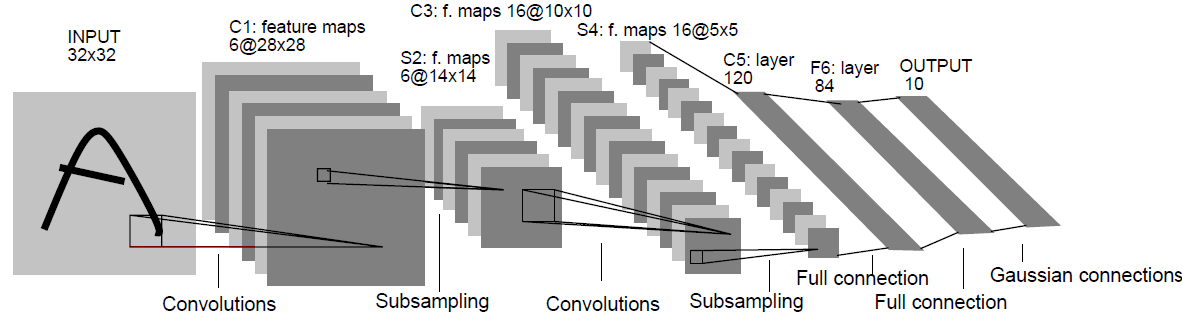
\includegraphics[width=0.85\textwidth]{figs/LeNet-5.png}
    \caption{Arhitectura LeNet-5, compusă din straturi convoluționale
    și de \textit{subsampling} alternante, urmate
    de straturi complet conectate \cite{lecun1998gradient}.}
    \label{fig:lenet5}
\end{figure}









\subsection{Componente fundamentale}

O rețea convoluțională este compusă, în mod tipic, dintr-o succesiune de blocuri convoluționale, urmate de unul sau mai multe straturi complet conectate care realizează clasificarea finală. Fiecare bloc convoluțional cuprinde, de regulă, mai multe tipuri de operații: convoluția propriu-zisă, normalizarea activărilor, funcția de activare neliniară și operația de agregare spațială (\textit{pooling}).

Stratul convoluțional aplică un set de filtre (\textit{kernels}) de dimensiuni reduse (de exemplu 3×3, 5×5 sau 11×11 pixeli) asupra imaginii de intrare, prin glisarea filtrului pe întreaga suprafață a imaginii și calcularea produsului scalar dintre ponderile filtrului și regiunea locală suprapusă la fiecare poziție. Fiecare filtru detectează un anumit tip de trăsătură vizuală: muchii, colțuri și texturi în straturile inferioare, forme și obiecte complexe în straturile superioare. Rezultatul aplicării unui filtru pe întreaga imagine formează o hartă de caracteristici (\textit{feature map}). Avantajul esențial al convoluției este partajarea ponderilor: același filtru este utilizat în toate pozițiile imaginii, ceea ce reduce drastic numărul de parametri ai modelului în comparație cu un strat complet conectat de aceeași dimensiune și introduce, în același timp, invarianța la translație.

Pe măsură ce rețelele convoluționale au devenit mai profunde, antrenarea lor a fost îngreunată de fenomenul \textit{internal covariate shift}: distribuția statistică a activărilor unui strat se modifică continuu pe parcursul antrenării, pe măsură ce ponderile straturilor anterioare sunt actualizate, ceea ce încetinește convergența și impune rate de învățare mai mici. O primă formă de normalizare a activărilor, introdusă chiar în arhitectura AlexNet \cite{krizhevsky2012imagenet}, este normalizarea locală a răspunsului (\textit{Local Response Normalization}, LRN), aplicată după funcția de activare ReLU în primele două straturi convoluționale și care reduce eroarea de clasificare cu 1.4 puncte procentuale pentru top-1 și 1.2 puncte procentuale pentru top-5 pe ILSVRC-2012. Câțiva ani mai târziu, normalizarea pe loturi (\textit{Batch Normalization}) \cite{ioffe2015batchnorm} a generalizat această idee, normalizând activările fiecărui strat la nivelul fiecărui mini-batch de antrenare, indiferent de poziția stratului în rețea, ceea ce permite utilizarea unor rate de învățare considerabil mai mari și o convergență mai rapidă. Datorită eficienței superioare, Batch Normalization a devenit standardul utilizat în arhitecturile convoluționale moderne, în locul LRN.

Ieșirea fiecărui strat convoluțional este trecută printr-o funcție de activare neliniară, cea mai utilizată în arhitecturile moderne fiind ReLU (\textit{Rectified Linear Unit}), definită ca $f(x) = \max(0, x)$ \cite{nair2010rectified}. Comparativ cu unitățile binare stocastice utilizate inițial în rețelele de tip Boltzmann, ReLU permite o reprezentare mai bogată a informației de intensitate și facilitează propagarea acesteia prin mai multe straturi de extragere a trăsăturilor \cite{nair2010rectified}.

După unul sau mai multe straturi convoluționale este frecvent aplicată o operație de pooling, care reduce dimensiunea spațială a hărților de caracteristici prin agregarea valorilor dintr-o vecinătate locală: de exemplu, {\it max-pooling} selectează valoarea maximă dintr-o fereastră de 2×2 sau 3×3 pixeli. Pooling-ul îndeplinește două roluri principale: reduce volumul de calcul necesar pentru straturile următoare și introduce un grad de invarianță la mici translații sau deformări ale obiectului din imagine.

O limitare importantă a rețelelor convoluționale foarte profunde este degradarea performanței la creșterea numărului de straturi, fenomen cauzat de dificultatea propagării gradientului prin multe straturi succesive. He et al. \cite{he2016resnet} au introdus conexiunile reziduale (\textit{skip connections}), prin care ieșirea unui bloc de straturi este adunată direct cu intrarea sa nemodificată, permițând gradientului să se propage mai facil înapoi prin rețea și făcând posibilă antrenarea unor arhitecturi cu sute de straturi.

După parcurgerea blocurilor convoluționale, reprezentarea extrasă este transmisă unor straturi complet conectate, similare celor dintr-o rețea neuronală clasică. Stratul final de ieșire este, în cazul problemelor de clasificare, activat printr-o funcție {\it softmax}, care transformă valorile brute de ieșire (\textit{logits}) într-o distribuție de probabilitate peste clasele posibile, astfel încât suma probabilităților asociate tuturor claselor să fie egală cu 1.


\subsection{Procesul de învățare}

Antrenarea unei rețele convoluționale constă în ajustarea iterativă a ponderilor modelului astfel încât predicțiile acestuia să se aproprie cât mai mult de etichetele reale ale datelor de antrenare. Acest proces necesită definirea unei funcții de pierdere (\textit{loss function}), care măsoară diferența dintre predicțiile modelului și etichetele corecte. Pentru probleme de clasificare, cea mai utilizată funcție de pierdere este entropia încrucișată (\textit{cross-entropy loss}), care penalizează cu atât mai mult o predicție cu cât probabilitatea atribuită clasei corecte este mai mică.

Minimizarea funcției de pierdere se realizează prin algoritmi de tip gradient descendent (\textit{gradient descent}), care actualizează ponderile modelului în direcția opusă gradientului funcției de pierdere în raport cu ponderile respective, calculat prin propagare inversă (\textit{backpropagation}). Algoritmul de bază, SGD (\textit{Stochastic Gradient Descent}), calculează gradientul pe subseturi mici de date (\textit{mini-batch-uri}) la fiecare pas de actualizare, în locul întregului set de antrenare, ceea ce reduce costul computațional și introduce un efect de regularizare prin natura sa stocastică. Implementările practice ale SGD includ frecvent un termen de momentum \cite{pytorch_sgd}, care acumulează o medie ponderată a gradienților anteriori pentru a stabiliza traiectoria de optimizare și a accelera convergența.

O alternativă larg utilizată este algoritmul Adam (\textit{Adaptive Moment Estimation}) \cite{kingma2014adam}, care adaptează rata de învățare individual pentru fiecare parametru al modelului, pe baza unor estimări ale primului și celui de-al doilea moment al gradienților. Adam converge frecvent mai rapid decât SGD clasic, în special pe seturi de date eterogene, dar poate fi mai predispus la suprapotrivire ({\it over-fitting}) pe seturi de date de dimensiuni reduse.

Performanța și comportamentul procesului de antrenare sunt influențate de o serie de hiperparametri (\textit{hyperparameters}), stabiliți înainte de antrenare și neactualizați prin procesul de propagare inversă. Dintre aceștia, cei mai importanți sunt rata de învățare (\textit{learning rate}), care controlează magnitudinea actualizărilor ponderilor la fiecare pas, și dimensiunea batch-ului (\textit{batch size}), care determină numărul de exemple utilizate pentru calcularea gradientului la o singură actualizare. O rată de învățare prea mare poate determina divergența procesului de optimizare, în timp ce o valoare prea mică poate conduce la o convergență excesiv de lentă sau la blocarea într-un minim local nesatisfăcător. Dimensiunea batch-ului influențează, de asemenea, calitatea estimării gradientului și capacitatea de generalizare a modelului rezultat, valori mai mici introducând un grad mai ridicat de zgomot stocastic, care poate favoriza, în anumite condiții, o generalizare mai bună.

Rata de învățare nu trebuie neapărat fixată pe întreaga durată a antrenării; ea poate fi ajustată dinamic printr-un planificator (\textit{scheduler}). O strategie frecvent utilizată în practică este reducerea ratei de învățare atunci când performanța modelului pe setul de validare stagnează pentru un număr fixat de epoci (\textit{ReduceLROnPlateau}) \cite{pytorch_reducelronplateau}, permițând o explorare inițială rapidă a spațiului de soluții, urmată de o rafinare mai precisă spre finalul antrenării.

Pentru a preveni supra-potrivirea (\textit{overfitting}), fenomen prin care modelul memorează particularitățile setului de antrenare în detrimentul capacității de generalizare, sunt utilizate frecvent tehnici de regularizare (\textit{regularization}). Dropout \cite{srivastava2014dropout} dezactivează aleatoriu o proporție din neuronii unui strat la fiecare pas de antrenare, forțând rețeaua să nu se bazeze excesiv pe combinații specifice de neuroni. O altă tehnică frecvent întâlnită este \textit{weight decay} \cite{krogh1991weightdecay}, care penalizează ponderile de magnitudine mare prin adăugarea unui termen proporțional cu norma acestora la funcția de pierdere, favorizând soluții mai simple și reducând riscul de supra-potrivire.  \textit{Label smoothing} \cite{szegedy2016labelsmoothing} este o tehnică similară, aplicată direct etichetelor de antrenare: în locul unei distribuții de probabilitate extreme (1 pentru clasa corectă, 0 pentru celelalte), se atribuie o probabilitate ușor redusă clasei corecte și o mică probabilitate reziduală celorlalte clase, reducând supra-încrederea modelului (\textit{overconfidence}) în predicțiile sale.



\section{Modele de clasificare a imaginilor}

\subsection{AlexNet}

În lucrarea \cite{krizhevsky2012imagenet}, Krizhevsky et al. prezintă arhitectura AlexNet, o rețea neuronală convoluțională profundă antrenată pe setul de date ImageNet LSVRC-2010, conținând 1.2 milioane de imagini distribuite în 1000 de clase. Lucrarea reprezintă un punct de referință în domeniul viziunii computerizate, demonstrând pentru prima dată că rețelele convoluționale profunde pot depăși semnificativ metodele clasice de extragere manuală a trăsăturilor pe seturi de date de mari dimensiuni.

Arhitectura propusă este compusă din cinci straturi convoluționale urmate de trei straturi complet conectate, ilustrate în Figura~\ref{fig:alexnet_cap2}. Primul strat convoluțional aplică 96 de filtre de dimensiune 11×11 cu pas 4 pe imaginile de intrare redimensionate la 224×224 pixeli. Straturile convoluționale ulterioare utilizează filtre de dimensiuni mai mici (5×5 și 3×3), cu operații de max-pooling intercalate pentru reducerea dimensiunii spațiale a hărților de caracteristici. Stratul de ieșire conține 1000 de neuroni, corespunzând celor 1000 de clase ImageNet, activați printr-o funcție softmax. Numărul total de parametri ai modelului depășește 60 de milioane.

\begin{figure}[H]
    \centering
    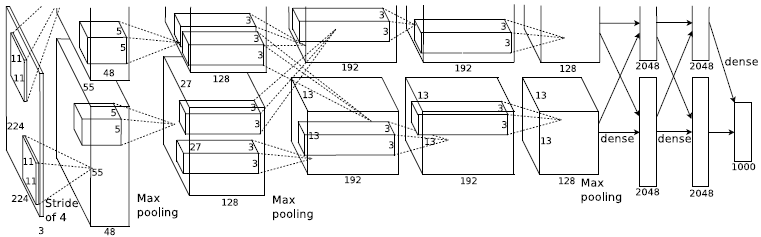
\includegraphics[width=\textwidth]{figs/AlexNetArhitectura.png}
    \caption{Arhitectura rețelei AlexNet cu cele cinci straturi
    convoluționale, operațiile de max-pooling și cele trei straturi
    complet conectate \cite{krizhevsky2012imagenet}.}
    \label{fig:alexnet_cap2}
\end{figure}

Lucrarea introduce mai multe contribuții tehnice care au devenit practici standard în deep learning. Funcția de activare ReLU (\textit{Rectified Linear Unit}) înlocuiește funcțiile sigmoidale clasice, accelerând convergența antrenării de câteva ori față de alternativele existente. Tehnica Dropout, aplicată cu o rată de 0.5 în straturile complet conectate, reduce supra-antrenarea prin dezactivarea aleatorie a neuronilor în timpul antrenării. Augmentarea datelor prin decupări și reflexii aleatorii ale imaginilor de antrenare contribuie suplimentar la regularizare. Antrenarea este realizată pe două unități GPU în paralel timp de cinci zile, utilizând metoda gradientului descendent stocastic cu moment.

Modelul a obținut o rată de eroare top-5 de 15.3\% pe setul de testare ILSVRC-2010, față de 26.2\% obținută de cel mai bun model alternativ din competiție, reprezentând o îmbunătățire de peste 10 puncte procentuale. Performanța a demonstrat că adâncimea rețelei este esențială: eliminarea oricăruia dintre straturile convoluționale intermediare conducea la degradarea semnificativă a acurateței.

Avantajele arhitecturii constau în capacitatea de a învăța automat reprezentări ierarhice ale trăsăturilor vizuale, de la muchii și texturi simple în straturile inferioare până la concepte semantice complexe în straturile superioare, fără a necesita inginerie manuală a trăsăturilor. Limitările includ numărul mare de parametri (peste 60 de milioane), care impune seturi de date mari pentru antrenare de la zero și resurse computaționale considerabile, precum și sensibilitatea la variațiile de iluminare și unghi în absența augmentării datelor.





\section{Modele pentru segmentarea imaginilor}

Segmentarea imaginilor reprezintă o categorie de sarcini de viziune computerizată
în care obiectivul este atribuirea unei etichete de clasă fiecărui pixel din imagine, spre diferență  de clasificare, unde se atribuie o singură etichetă întregii imagini, sau de detecția obiectelor, unde obiectele sunt localizate prin dreptunghiuri de încadrare. Rezultatul unei segmentări este o hartă de aceeași rezoluție cu imaginea de intrare, în care fiecare pixel este asociat clasei obiectului din care face parte, permițând o delimitare precisă a formei și conturului obiectelor de interes. Această granularitate ridicată face din segmentare o sarcină considerabil mai complexă din punct de vedere computațional decât clasificarea, dar și mult mai informativă pentru aplicații care necesită localizarea exactă a obiectelor, precum imagistica medicală sau analiza scenelor naturale.

\subsection{U-Net}

U-Net \cite{ronneberger2015unet} este una dintre cele mai influente arhitecturi dezvoltate pentru segmentare, propusă inițial pentru segmentarea imaginilor biomedicale.

Arhitectura U-Net este organizată simetric, sub forma literei U, fiind compusă din două componente principale: un {\it encoder} (calea de contractare), care extrage progresiv trăsături printr-o succesiune de straturi convoluționale și operații de pooling, reducând dimensiunea spațială a reprezentării, și un {\it decoder} (calea de expansiune), care reconstruiește dimensiunea spațială originală prin operații de up-sampling, generând în final o hartă de segmentare de aceeași rezoluție cu imaginea de intrare. Particularitatea esențială a U-Net constă în conexiunile directe (\textit{skip connections}) dintre straturile corespunzătoare ale encoder-ului și decoder-ului, prin care trăsăturile de detaliu spațial, pierdute parțial în procesul de contractare, sunt transmise direct către decoder, permițând o localizare mai precisă a obiectelor segmentate. O altă caracteristică notabilă a arhitecturii este capacitatea sa de a obține rezultate competitive folosind seturi de date de antrenare relativ mici, proprietate care a contribuit la adoptarea sa pe scară largă în domenii unde adnotarea pixel-cu-pixel este costisitoare, precum imagistica medicală. Structura arhitecturii este ilustrată în Figura~\ref{fig:unet}.

\begin{figure}[htbp]
    \centering
    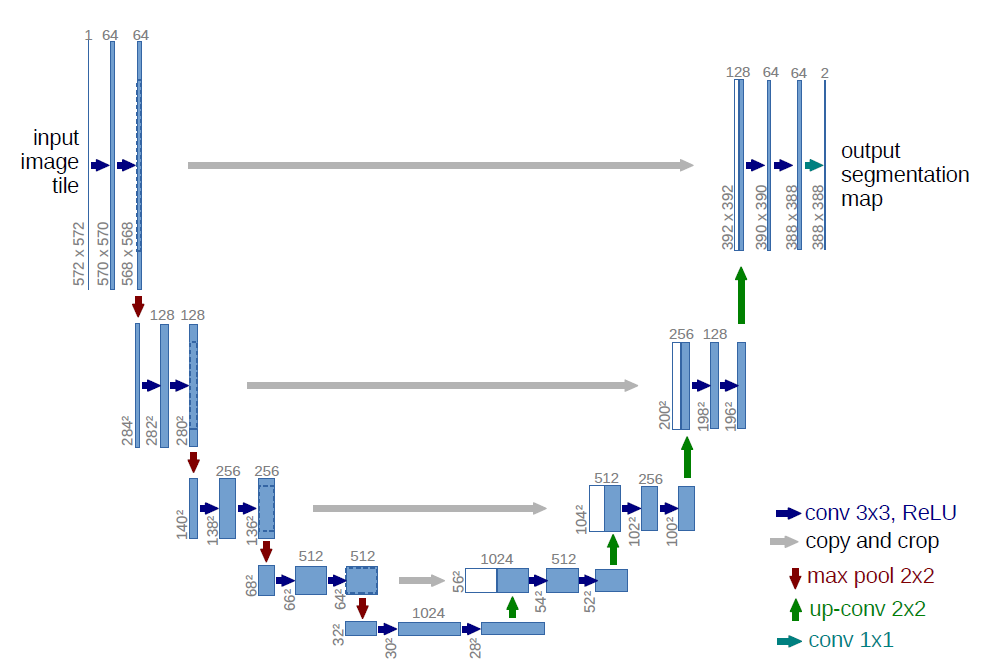
\includegraphics[width=\textwidth]{figs/UNetArhitectura.png}
    \caption{Arhitectura U-Net, ilustrând organizarea simetrică în
    formă de U a encoder-ului și decoder-ului \cite{ronneberger2015unet}.}
    \label{fig:unet}
\end{figure}

\subsection{ResNet}

Pe măsură ce rețelele convoluționale destinate clasificării au crescut în profunzime, cercetătorii au observat un fenomen de degradare a performanței: dincolo de un anumit număr de straturi, adăugarea de straturi suplimentare nu mai aducea o creștere a acurateței, ci, dimpotrivă, o deteriora, fenomen distinct de simpla suprapotrivire. Cauza principală este dificultatea propagării gradientului prin un număr mare de straturi succesive în procesul de propagare inversă. He et al. \cite{he2016resnet} au adresat această problemă prin introducerea arhitecturii ResNet (\textit{Residual Network}), bazată pe blocuri reziduale: în loc ca un bloc de straturi să învețe direct funcția de transformare dorită, acesta învață doar diferența (\textit{reziduul}) față de intrarea sa, care este adunată direct la ieșire printr-o conexiune reziduală. Această reformulare facilitează considerabil propagarea gradientului către straturile inferioare, permițând antrenarea unor rețele cu sute de straturi, comparativ cu câteva zeci de straturi posibile anterior. Cea mai profundă variantă propusă de autori, cu 152 de straturi, a obținut o eroare de doar 3,57\% pe setul de testare ImageNet, câștigând competiția ILSVRC din 2015. Structura blocului rezidual de bază este ilustrată în Figura~\ref{fig:resnet_block}, iar Figura~\ref{fig:resnet_arch} prezintă modul în care aceste blocuri sunt integrate într-o arhitectură completă, prin comparație cu o rețea convoluțională simplă de profunzime echivalentă.

\begin{figure}[htbp]
    \centering
    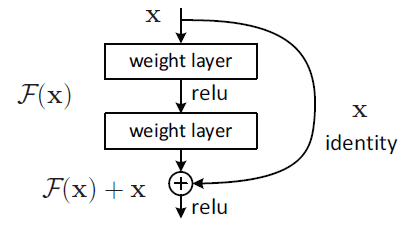
\includegraphics[width=0.5\textwidth]{figs/ResNetBlocRezidual.png}
    \caption{Blocul rezidual de bază propus de He et al.
    \cite{he2016resnet}.}
    \label{fig:resnet_block}
\end{figure}

\begin{figure}[htbp]
    \centering
    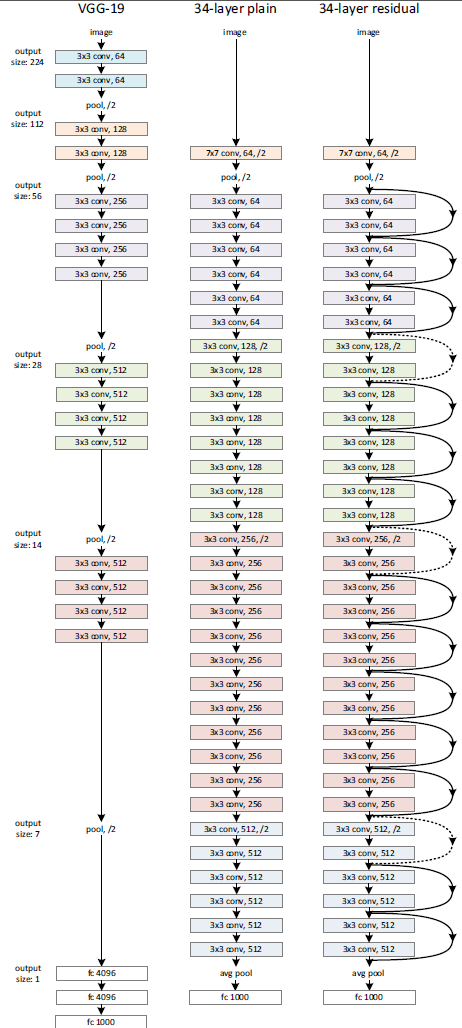
\includegraphics[height=0.85\textheight]{figs/ResNetArhitectura.png}
    \caption{Comparație între arhitectura VGG-19, o rețea
    convoluțională simplă cu 34 de straturi (\textit{34-layer plain})
    și varianta reziduală echivalentă (\textit{34-layer residual}),
    evidențiind conexiunile reziduale introduse la fiecare pereche
    de straturi \cite{he2016resnet}.}
    \label{fig:resnet_arch}
\end{figure}

\subsection{EfficientNet}

O direcție alternativă de dezvoltare a arhitecturilor convoluționale moderne s-a concentrat nu pe introducerea unor module noi, ci pe modul în care o arhitectură de bază este scalată pentru a obține performanțe superioare. Practica obișnuită înainte de  EfficientNet consta în scalarea arbitrară a unei singure dimensiuni a rețelei, fie prin creșterea profunzimii (numărul de straturi), fie a lățimii (numărul de filtre per strat), fie a rezoluției imaginilor de intrare. Tan și Le \cite{tan2019efficientnet} au demonstrat că o scalare echilibrată și simultană a tuturor celor trei dimensiuni, printr-un coeficient compus (\textit{compound scaling}) determinat printr-o căutare sistematică pe o arhitectură de bază, conduce la un raport considerabil mai favorabil între acuratețe și costul computațional decât scalarea independentă a unei singure dimensiuni. Familia de modele rezultată, EfficientNet, obține o acuratețe comparabilă sau superioară arhitecturilor anterioare, folosind un număr semnificativ mai redus de parametri, varianta cea mai performantă (EfficientNet-B7) atingând 84,3\% acuratețe top-1 pe ImageNet. Cele patru strategii de scalare, alături de scalarea compusă propusă, sunt ilustrate comparativ în Figura~\ref{fig:efficientnet}.

\begin{figure}[H]
    \centering
    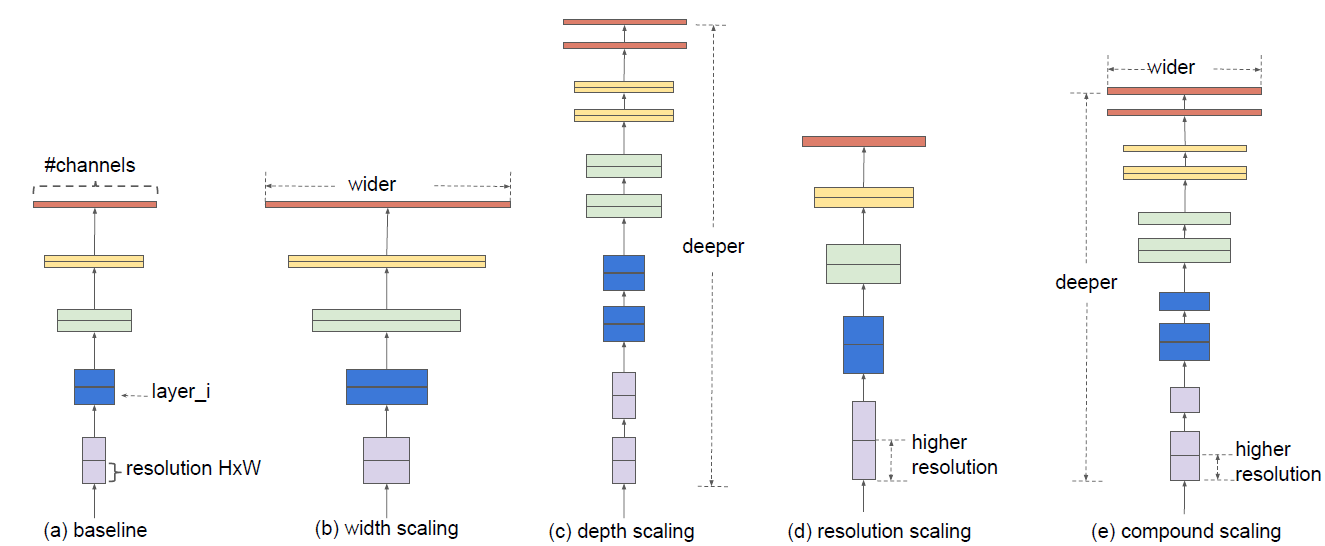
\includegraphics[width=\textwidth]{figs/EfficientNetScaling.png}
    \caption{Strategii de scalare a unei rețele convoluționale:
    referință (a), scalare în lățime (b), scalare în profunzime (c),
    scalare a rezoluției (d) și scalarea compusă (\textit{compound
    scaling}) propusă de EfficientNet (e) \cite{tan2019efficientnet}.}
    \label{fig:efficientnet}
\end{figure}







\section{Modele pentru identificarea obiectelor din imagini}

Detecția obiectelor este o sarcină intermediară între clasificare și segmentare: scopul nu este doar atribuirea unei etichete imaginii, ca în clasificare, dar nici delimitarea exactă a fiecărui pixel, ca în segmentare, ci localizarea obiectelor de interes prin dreptunghiuri de încadrare (\textit{bounding boxes}), însoțite de eticheta clasei corespunzătoare. Abordările anterioare anului 2016 tratau, în general, detecția în mai multe etape: o primă etapă propunea regiuni candidate din imagine, urmată de o etapă separată de clasificare a fiecărei regiuni propuse, ceea ce făcea procesul lent și dificil de optimizat de la un cap la altul.

YOLO (\textit{You Only Look Once}) \cite{redmon2016yolo} a schimbat fundamental această abordare, reformulând detecția ca o problemă unică de regresie. Imaginea de intrare este împărțită într-un grid de celule, iar pentru fiecare celulă o singură rețea convoluțională prezintă direct coordonatele dreptunghiurilor de încadrare și probabilitățile de clasă asociate, totul într-o singură trecere prin rețea. Această abordare unificată elimină nevoia unei etape separate de propunere a regiunilor candidate și permite optimizarea întregului proces de detecție direct pe performanța finală, aducând YOLO un avantaj considerabil de viteză: varianta originală a modelului prelucrează imagini la 45 de cadre pe secundă, suficient pentru detecție în timp real. Figura~\ref{fig:yolo_system} ilustrează fluxul general al sistemului de detecție, Figura~\ref{fig:yolo_model} detaliază modul în care gridul de celule generează dreptunghiurile de încadrare și harta probabilităților de clasă, iar Figura~\ref{fig:yolo_arch} prezintă arhitectura completă a rețelei convoluționale utilizate.

\begin{figure}[H]
    \centering
    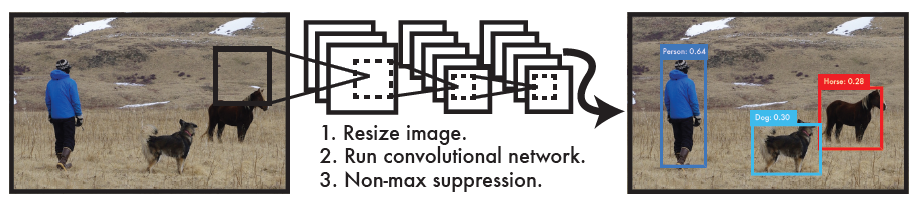
\includegraphics[width=\textwidth]{figs/YOLODetectionSystem.png}
    \caption{Sistemul de detecție YOLO: cei trei pași ai procesării,
    de la imaginea de intrare la detecțiile finale
    \cite{redmon2016yolo}.}
    \label{fig:yolo_system}
\end{figure}

\begin{figure}[H]
    \centering
    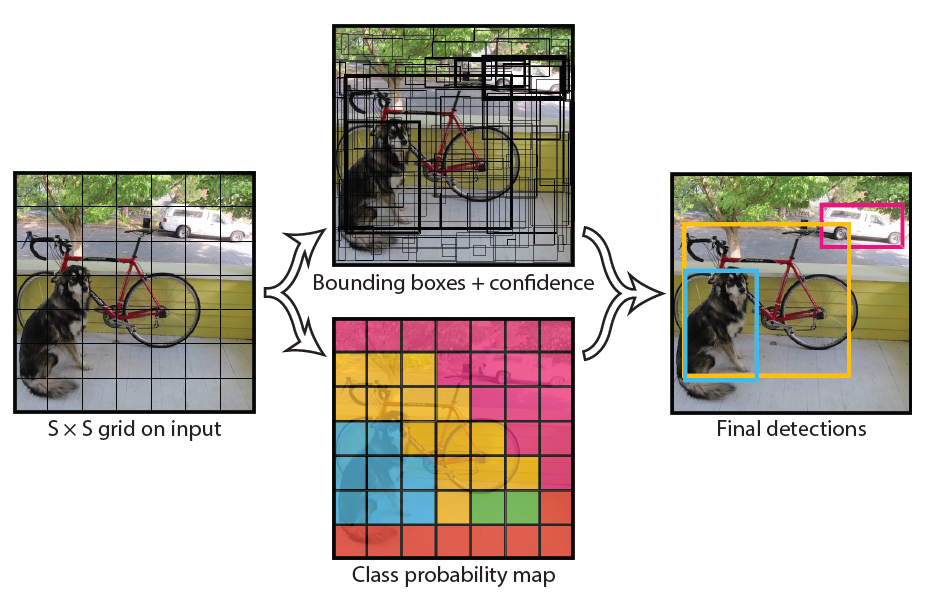
\includegraphics[width=0.75\textwidth]{figs/YOLOModel.png}
    \caption{Modelul YOLO: imaginea este împărțită într-un grid
    $S \times S$, pentru fiecare celulă fiind prezise dreptunghiuri
    de încadrare cu scoruri de încredere asociate și o hartă a
    probabilităților de clasă, combinate în detecțiile finale
    \cite{redmon2016yolo}.}
    \label{fig:yolo_model}
\end{figure}

\begin{figure}[H]
    \centering
    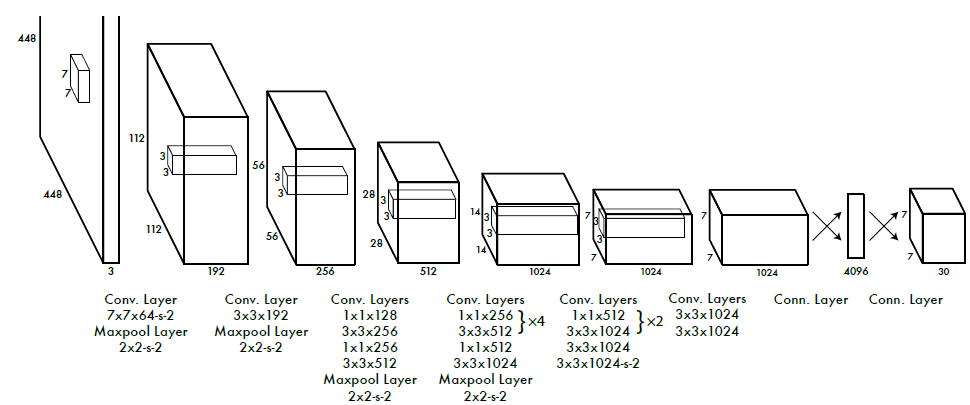
\includegraphics[width=\textwidth]{figs/YOLOArhitectura.png}
    \caption{Arhitectura rețelei YOLO, compusă din 24 de straturi
    convoluționale urmate de 2 straturi complet conectate. Straturile
    de reducere $1\times1$, alternate cu straturi convoluționale
    $3\times3$, reduc numărul de canale înainte de procesarea spațială
    ulterioară \cite{redmon2016yolo}.}
    \label{fig:yolo_arch}
\end{figure}

De la publicarea variantei inițiale, arhitectura YOLO a fost extinsă și rafinată în numeroase versiuni succesive, fiecare aducând îmbunătățiri la nivelul vitezei, acurateței sau dimensiunii modelului. Capitolul \ref{chapter:cap3} discută în detaliu două astfel de versiuni, YOLOv11n și YOLOv8n, aplicate specific pe sarcina detecției și segmentării specimenelor de raci de apă dulce, ilustrând modul în care principiul de bază introdus de YOLO a fost adaptat pentru aplicații practice de monitorizare a biodiversității acvatice.












% arhitectura
% nuclee de convoluție (kernels), module de agregare și redimensionare (pooling), nivel de clasificare (softmax)
% proces de învățare:  funcție de eroare, algoritmi de antrenare (SGD, ADAM, etc), hiperparametri (batch size, learning rate etc)
%\section{Modele pentru segmentarea imaginilor}
% UNet
% ResNet
% EfficientNet
%\section{Modele pentru identificarea obiectelor din imagini}
% YOLO


\chapter{Descrierea problemei și abordări existente}\label{chapter:cap3} %{Materiale și metodă}

Acest capitol detaliază particularitățile problemei de clasificare abordate în lucrare, punând accent pe similaritățile morfologice pronunțate dintre cele două specii vizate și pe dificultățile pe care acestea le generează în procesul de identificare. Este realizată, în continuare, o analiză critică a unor lucrări recente din literatură care abordează probleme conexe de identificare automată a racilor prin tehnici de deep learning, bazate pe arhitecturi din familia YOLO. Pentru fiecare lucrare discutată sunt prezentate metodologia, rezultatele obținute și principalele limitări, urmate de o comparație explicită cu modul în care abordarea propusă în această lucrare se diferențiază prin natura problemei, speciile vizate și condițiile de colectare a datelor.

\section{Particularități ale problemei}

Identificarea speciilor de rac din imagini depinde de evidențierea caracteristicilor morfologice relevante, precum forma rostrului, structura cleștilor și conturul cefalotoracelui \cite{parvulescu2009}. Vizibilitatea acestor elemente este influențată de unghi, lumină și calitatea imaginii.

Cele două specii vizate, \textit{Austropotamobius bihariensis} și \textit{Austropotamobius torrentium}, prezintă similarități morfologice pronunțate: ambele au crusta netedă, creasta postorbitală discretă fără spin și rostrul de formă triunghiulară \cite{parvulescu2009}. Diferențele constau în detalii fine, precum lungimea relativă a solzului antenal față de articolele bazale ale antenei și gradul de rugozitate al chelelor, caractere care nu sunt vizibile în toate imaginile, în special atunci când exemplarul este parțial acoperit sau capturat dintr-un unghi nefavorabil.

Asemănările morfologice dintre specii impun analiza unor detalii fine, care nu sunt vizibile în toate imaginile. Identificarea corectă presupune localizarea regiunilor relevante și extragerea trăsăturilor utile pentru clasificare. O dificultate suplimentară este reprezentată de variabilitatea intraspecifică de colorit: \textit{A. torrentium} poate varia de la brun-închis la portocaliu-deschis sau chiar albicios \cite{parvulescu2009}, ceea ce reduce fiabilitatea culorii ca trăsătură discriminatorie și crește importanța caracteristicilor de formă și textură.


Figura~\ref{fig:specii_raci} ilustrează exemplare reprezentative din cele două specii, evidențiind atât similaritatea morfologică generală, cât și variabilitatea de colorit discutată anterior.

\begin{figure}[H]
    \centering
    \begin{subfigure}{0.45\textwidth}
        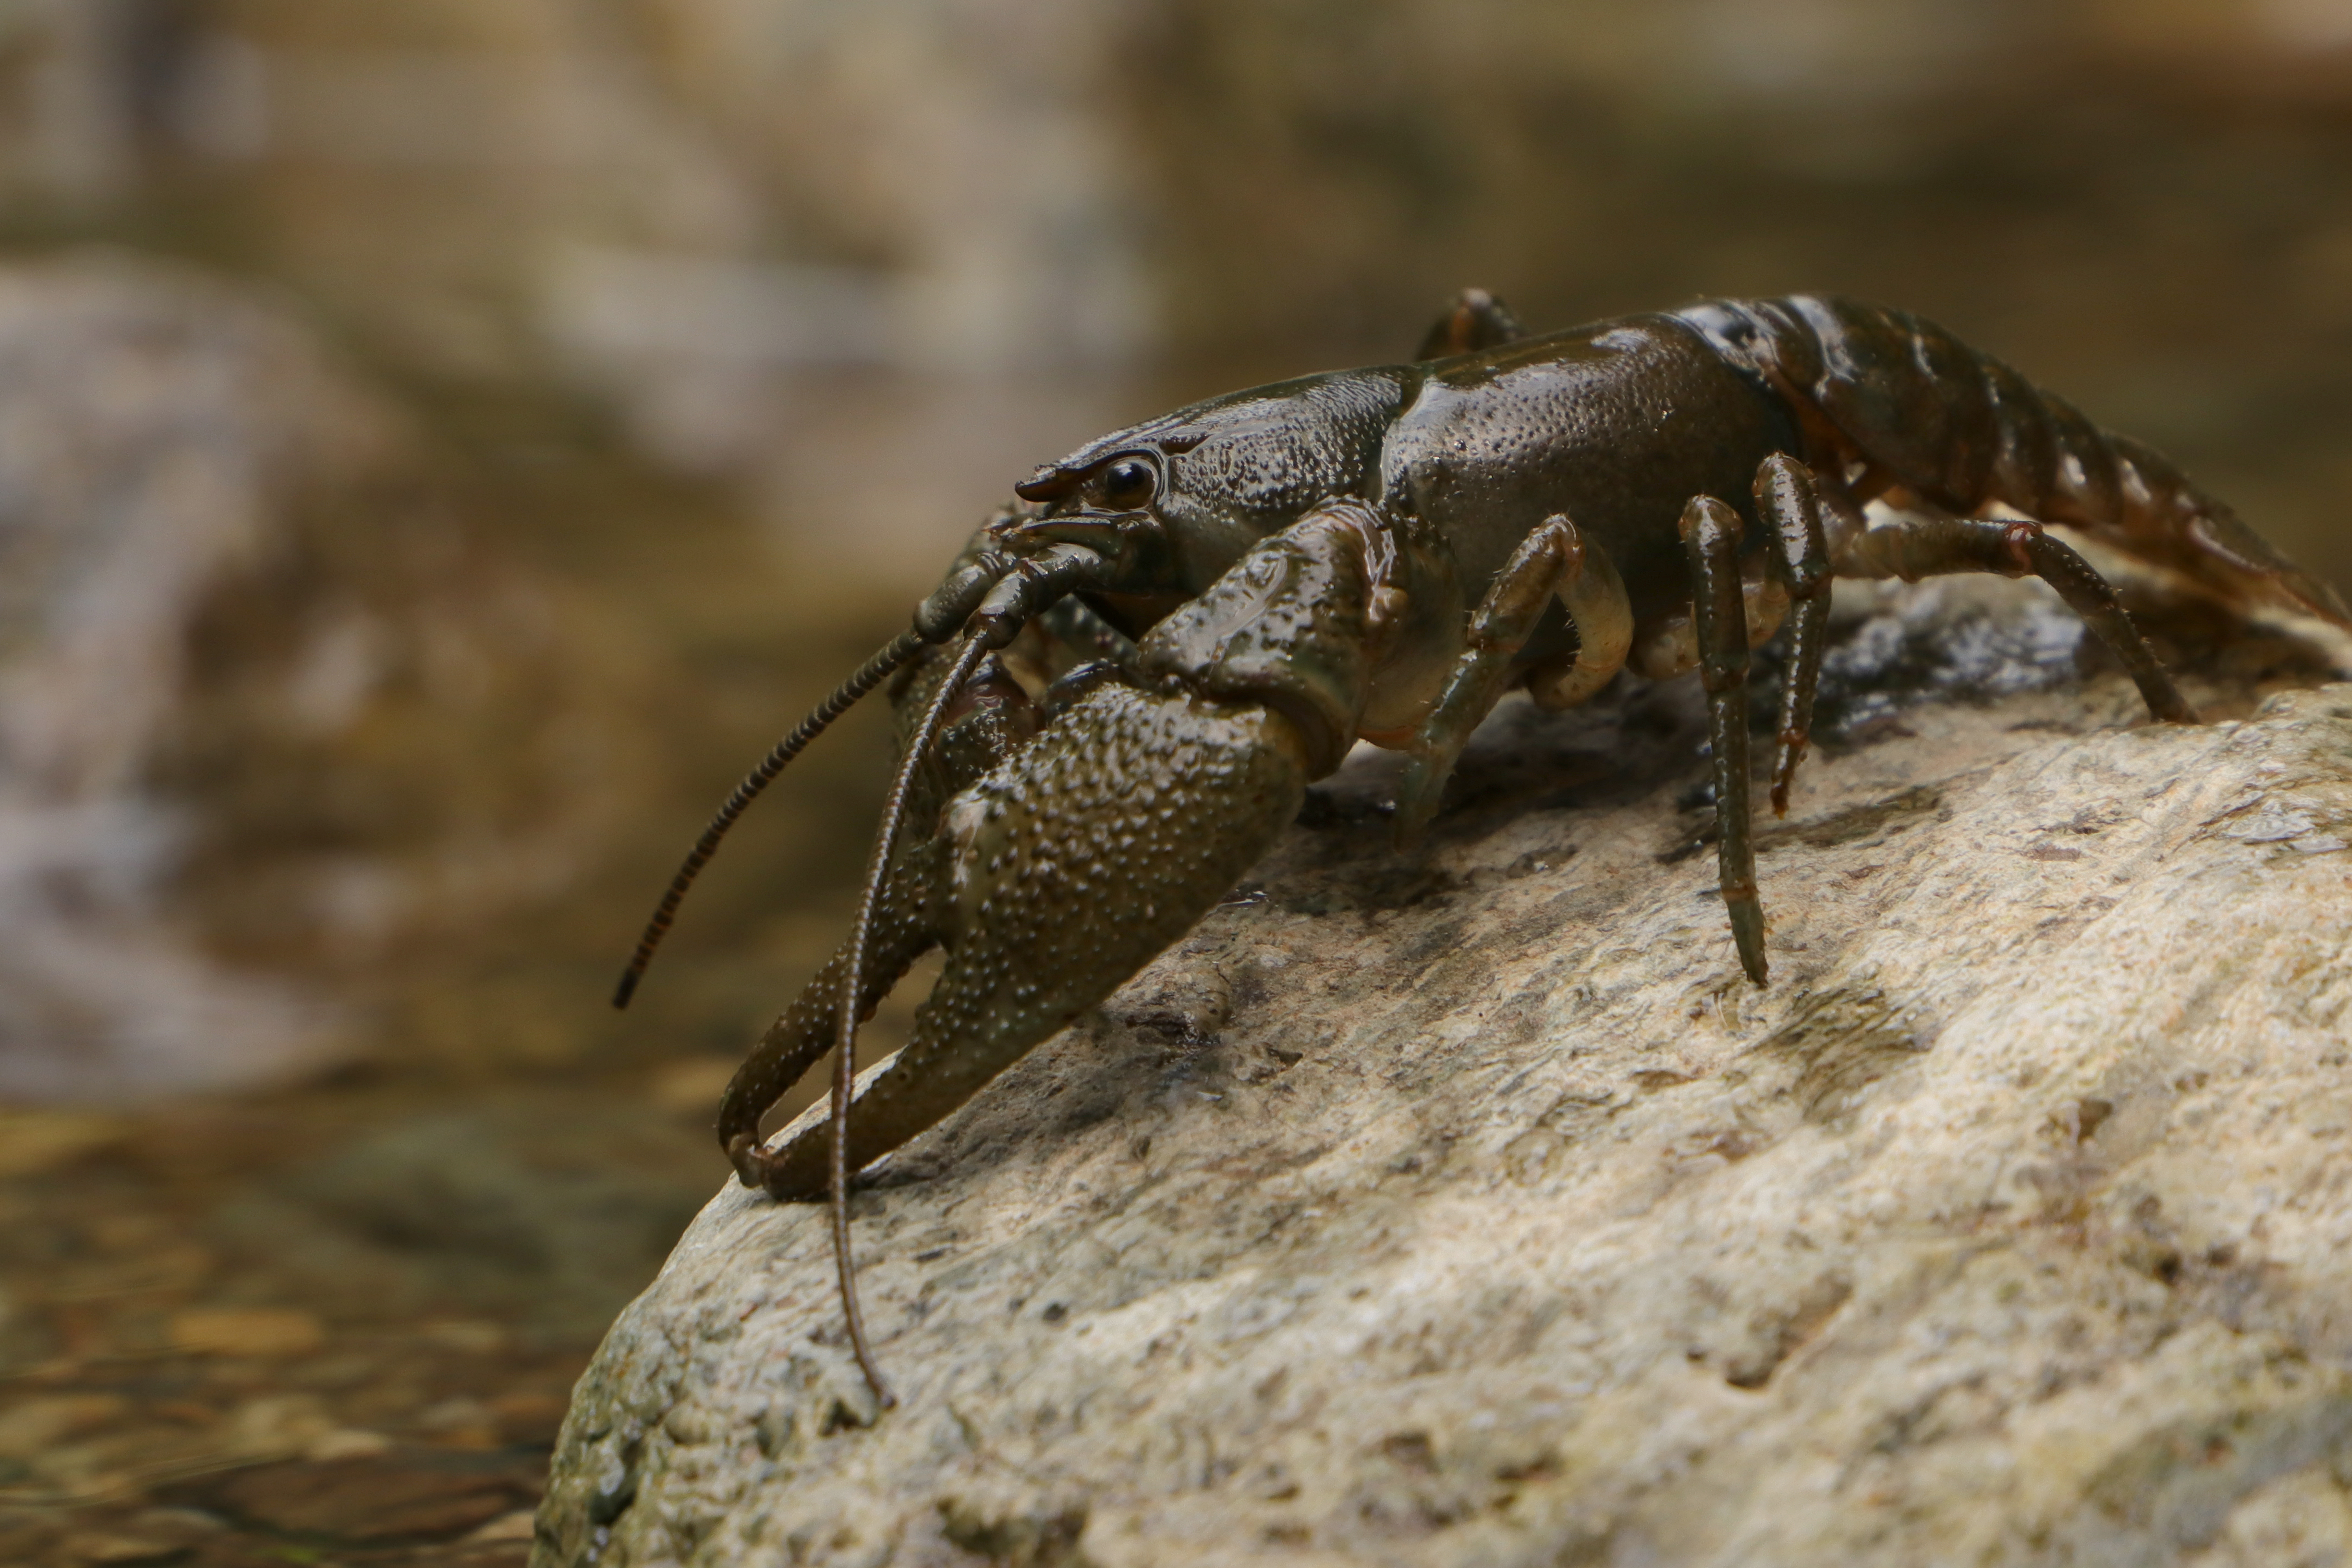
\includegraphics[width=\textwidth]{figs/Bihariensis_ex1.jpg}
    \end{subfigure}
    \hfill
    \begin{subfigure}{0.45\textwidth}
        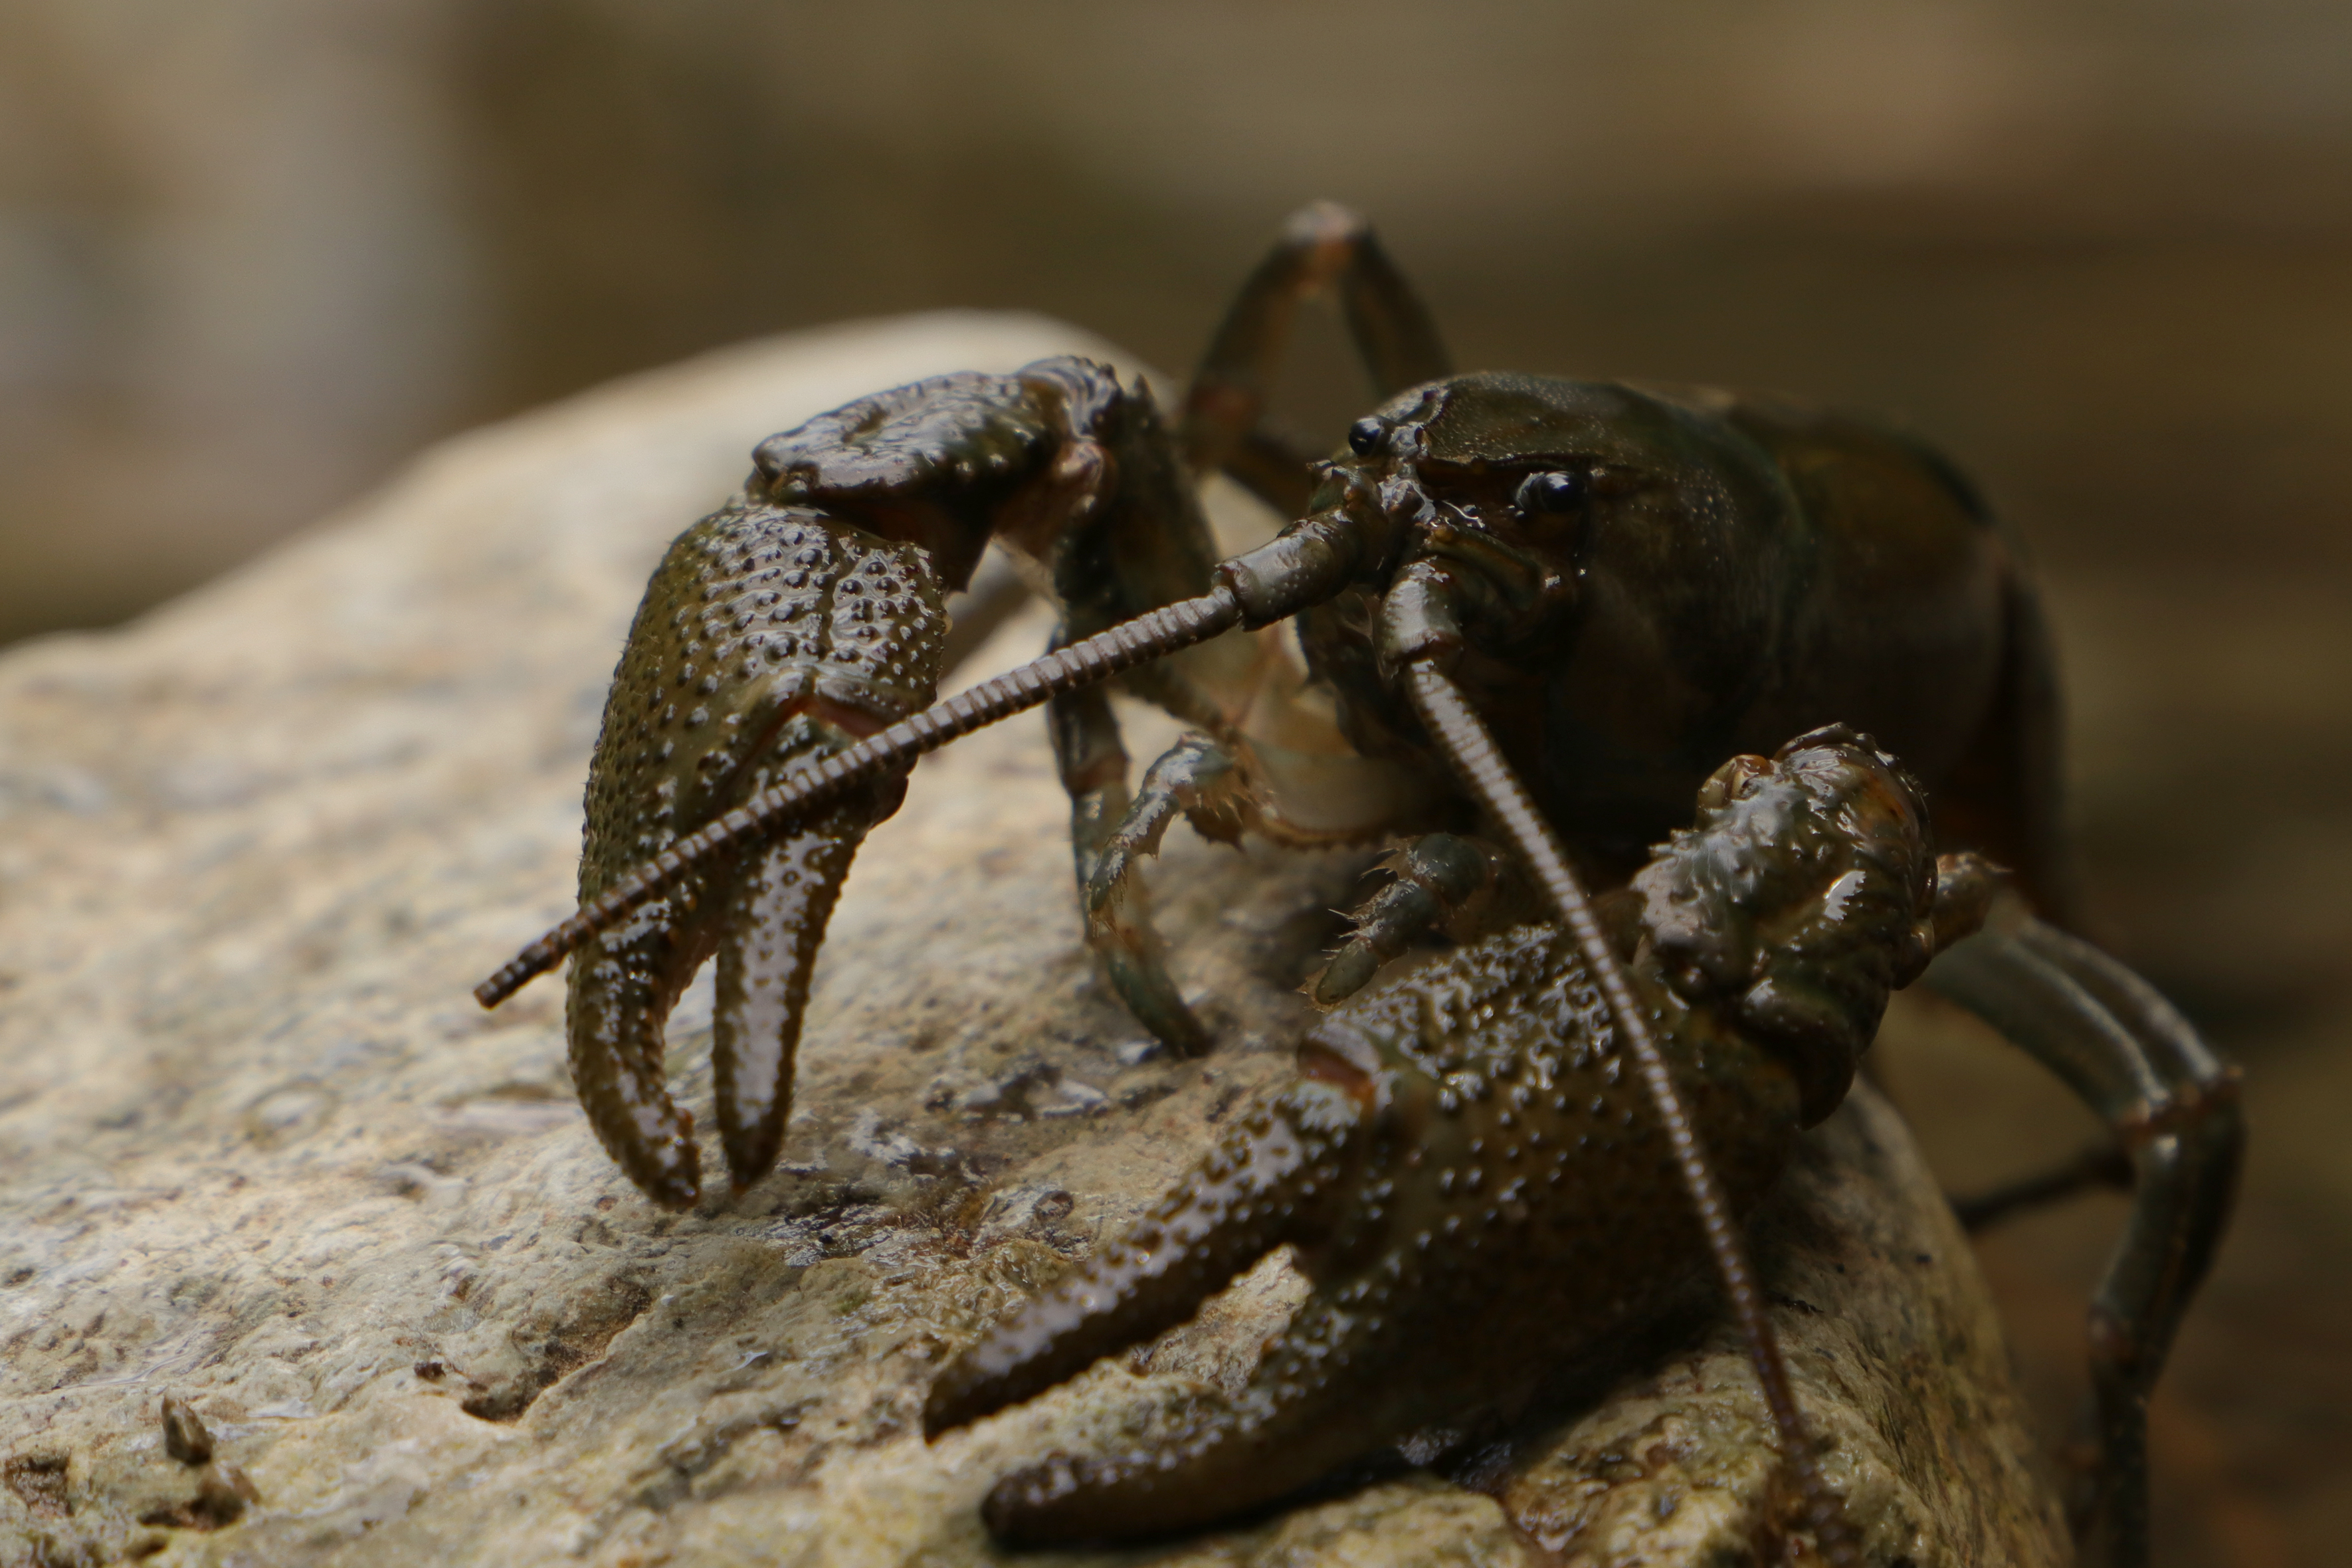
\includegraphics[width=\textwidth]{figs/Bihariensis_ex2.jpg}
    \end{subfigure}

    \vspace{0.5em}

    \begin{subfigure}{0.45\textwidth}
        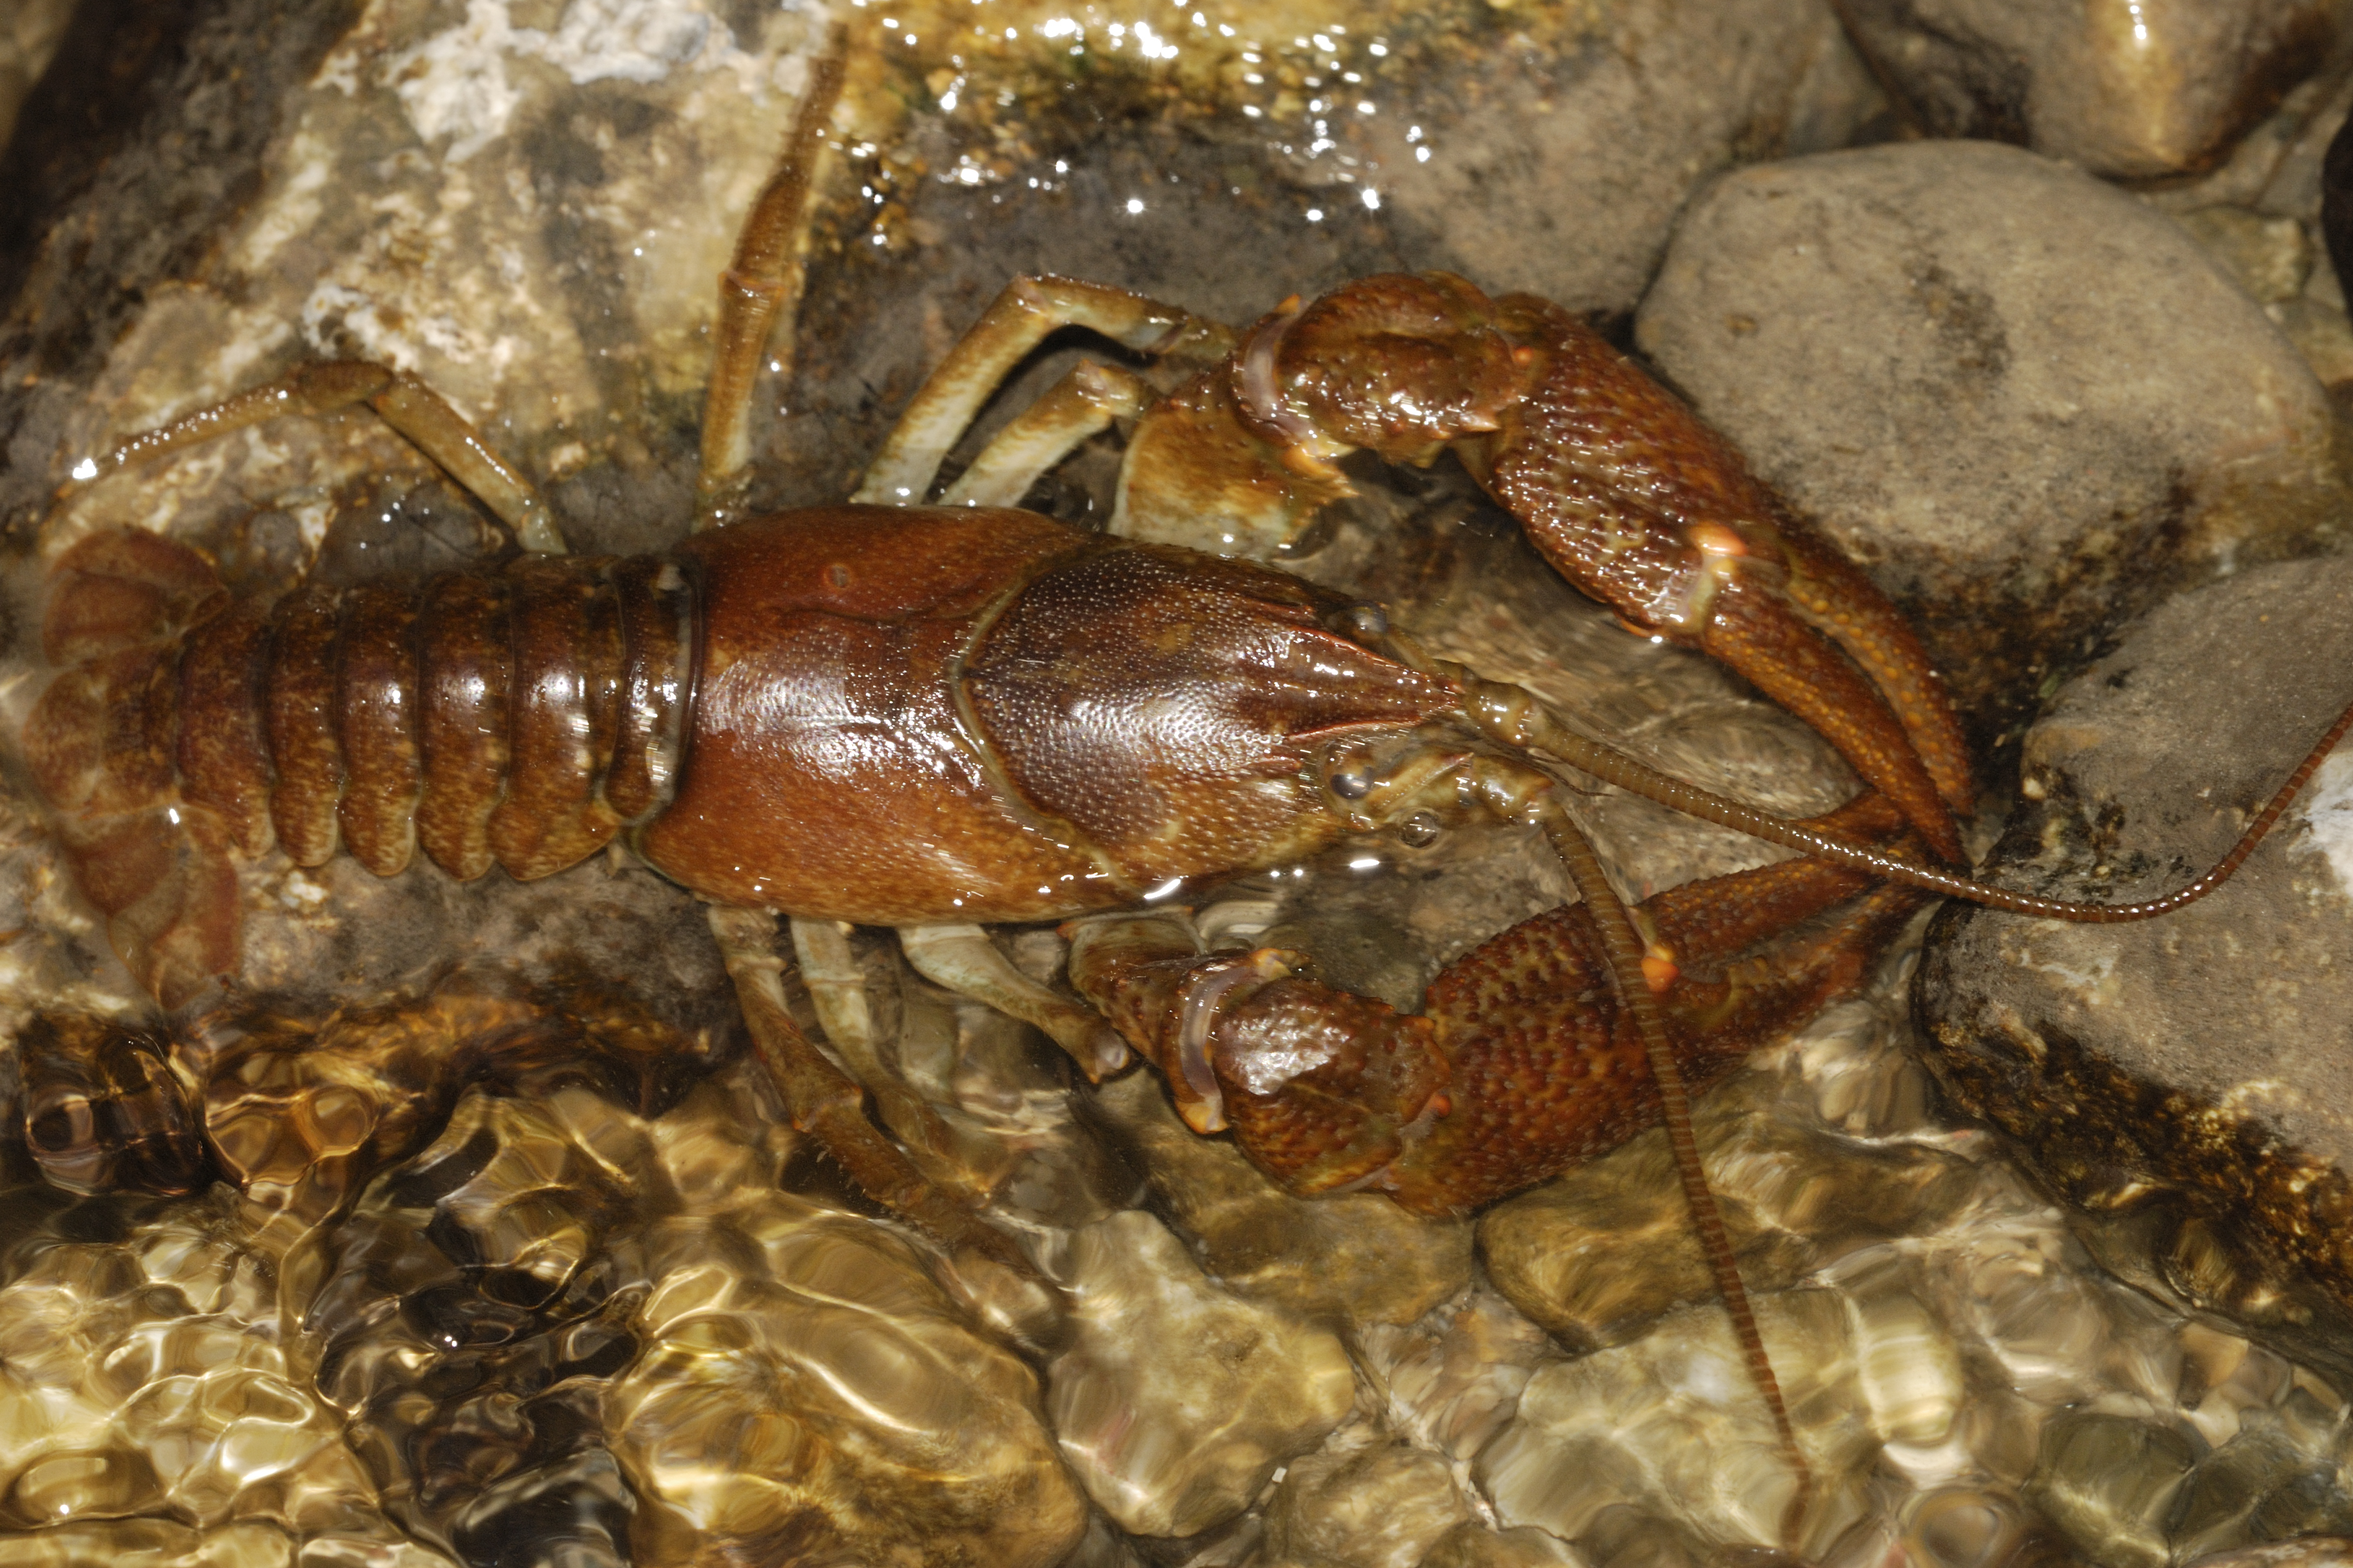
\includegraphics[width=\textwidth]{figs/Torrentium_ex1.jpg}
    \end{subfigure}
    \hfill
    \begin{subfigure}{0.45\textwidth}
        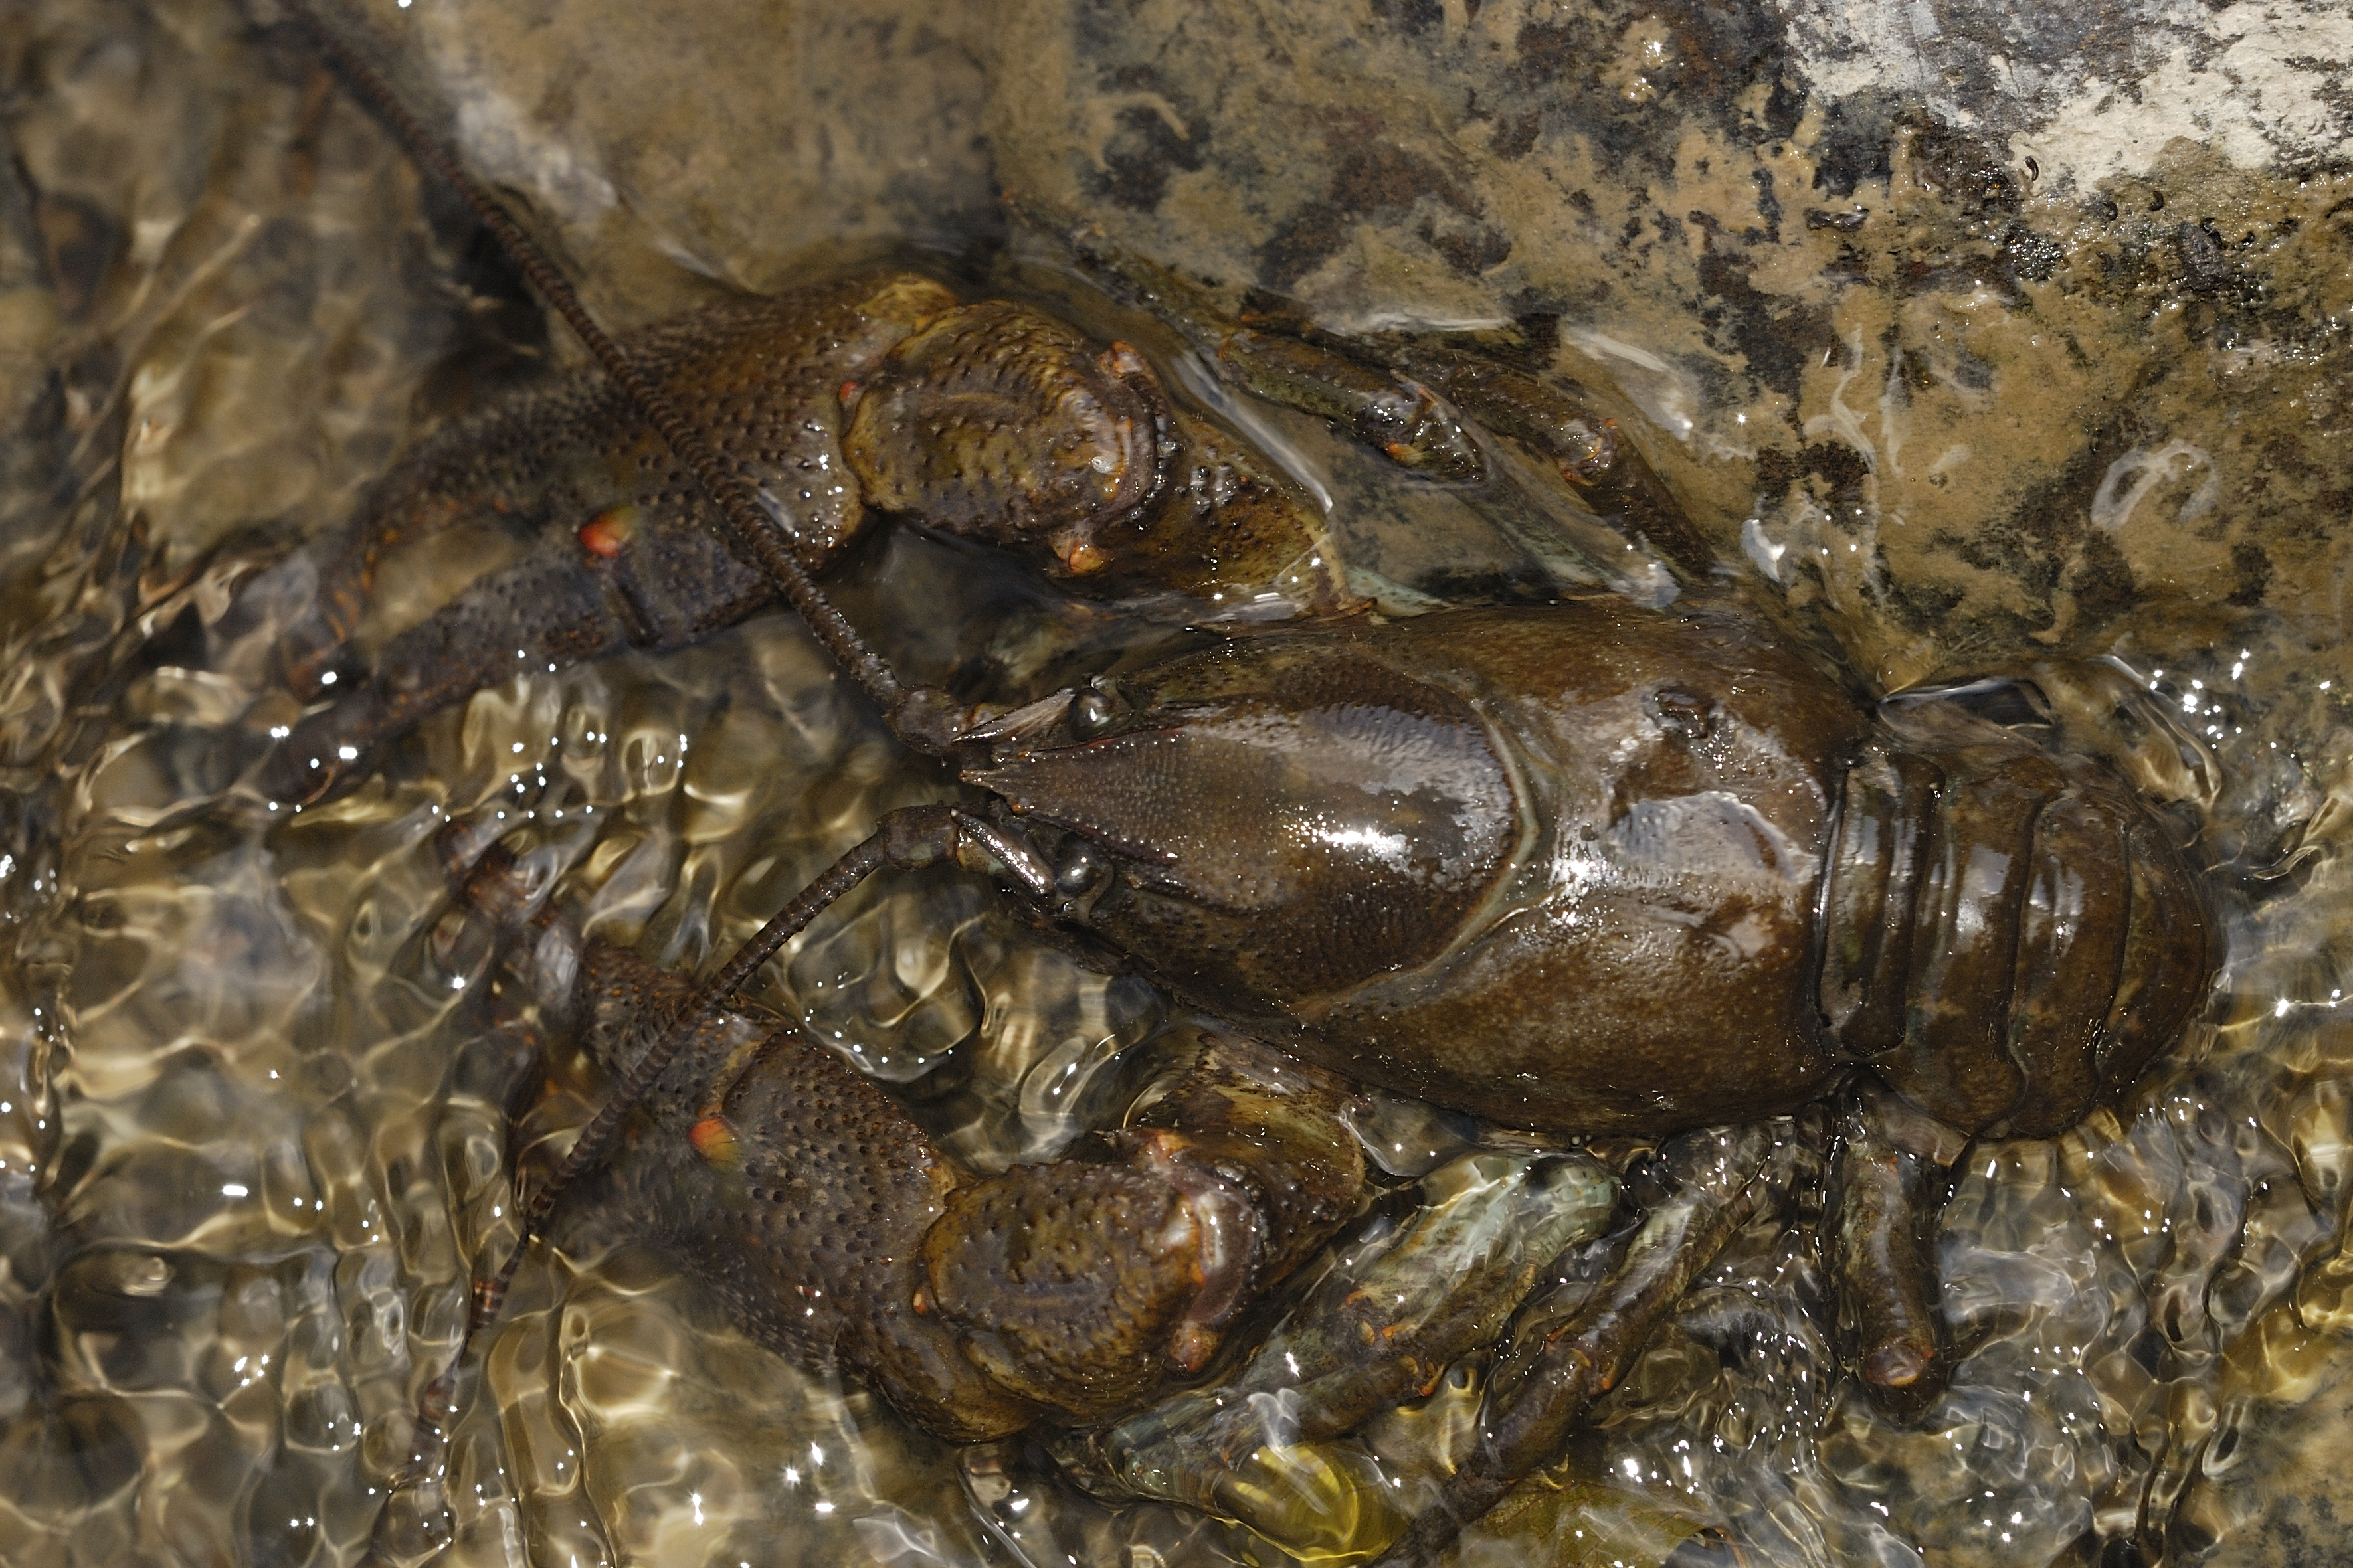
\includegraphics[width=\textwidth]{figs/Torrentium_ex2.jpg}
    \end{subfigure}
        \caption{Exemplare reprezentative de \textit{Austropotamobius
        bihariensis} (sus) și \textit{Austropotamobius torrentium} (jos),
        fotografiate în habitatul natural.}
    \label{fig:specii_raci}
\end{figure}



% exemple de imagini și caracteristici urmarite
% dificultati 
% exemple de imagini care pot conduce la concluzii
\section{Abordări existente}


Această secțiune prezintă lucrări recente în care sunt abordate probleme corelate cu cea studiată în această lucrare, axate pe identificarea automată a racilor prin tehnici de deep learning.


\subsection{Lightweight detection and segmentation of crayfish parts using an improved YOLOv11n model}

În lucrarea \cite{Lightweight_detection_and_segmentation_of_crayfish_parts_using_an_improved_YOLOv11n_segmentation_model}, autorii abordează problema detecției și segmentării sub-părților racilor (\textit{Procambarus clarkii}) în contexte industriale, unde este necesară o identificare precisă și rapidă a componentelor anatomice, precum cleștii, abdomenul, cefalotoracele și picioarele locomotoare. Problema este dificilă din cauza dimensiunilor reduse ale unor structuri, a ocluziilor frecvente și a scenelor aglomerate în care mai mulți indivizi se suprapun.

Metodologia propusă se bazează pe un model îmbunătățit de tip YOLOv11n-Seg (\textit{You Only Look Once version 11 nano -- Segmentation}), denumit YOLOv11n-DHBC. Autorii construiesc un set de date propriu, format inițial din 585 de imagini capturate la o rezoluție de 4032×3024 pixeli, utilizând un dispozitiv mobil, extins ulterior prin tehnici de augmentare la 3510 imagini. Setul de date este împărțit în subseturi de antrenare, validare și testare în raport 7:2:1, pentru a asigura o evaluare riguroasă a performanței modelului. Sunt definite patru clase de segmentare: cefalotorace, abdomen, clești și picioare locomotoare. Datele sunt etichetate manual la nivel de pixel folosind instrumentul LabelMe \cite{labelme} același instrument utilizat și în cadrul acestei lucrări pentru adnotarea imaginilor de rac.

Modelul introduce trei îmbunătățiri principale față de arhitectura de bază YOLOv11n-Seg: (1) un backbone D-HGNetV2 (\textit{Dynamic Hierarchical Graph Network version 2}), care integrează convoluții dinamice pentru o mai bună adaptare la variațiile datelor, reducând numărul de parametri cu 31\% față de modelul original; (2) un modul BiFPN (\textit{Bidirectional Feature Pyramid Network}) \cite{tan2020efficientdet}, utilizat pentru fuziunea bidirecțională a caracteristicilor multi-scală, cu ponderi învățabile care permit rețelei să determine autonom importanța fiecărei scări de reprezentare; și (3) un modul CARAFE (\textit{Content-Aware ReAssembly of FEatures}) \cite{wang2019carafe}, utilizat pentru upsampling adaptiv în locul interpolării nearest-neighbor clasice, care păstrează detaliile fine ale obiectelor mici.

Rezultatele experimentale arată că modelul propus atinge o performanță ridicată, obținând un mAP@0.5 de 96.8\% pentru detecție prin bounding box și 96.0\% pentru segmentare la nivel de instanță, depășind astfel performanțele modelului de bază YOLOv11n-Seg. Modelul este eficient din punct de vedere computațional, având doar 2.0 milioane de parametri și o dimensiune de 4.2 MB, putând rula în timp real la 65.8 cadre pe secundă (FPS).

Avantajele metodei includ un echilibru bun între acuratețe și eficiență, capacitatea de a gestiona obiecte mici și ocluzionate, precum și posibilitatea de implementare pe dispozitive cu resurse limitate (\textit{edge devices}). Limitările constau în dificultăți persistente în segmentarea completă a structurilor anatomice foarte mici în scenarii extrem de aglomerate și în dependența de un set de date specific domeniului industrial.

Comparativ cu alte metode evaluate, precum Mask R-CNN, YOLOv5s, YOLOv7 și YOLOv8n, modelul propus oferă o performanță similară sau superioară în termeni de acuratețe, cu un cost computațional considerabil mai redus, acesta fiind mai adecvat pentru aplicații industriale în timp real.

Față de abordarea prezentată în această lucrare, metoda propusă de Shi et al. \cite{Lightweight_detection_and_segmentation_of_crayfish_parts_using_an_improved_YOLOv11n_segmentation_model} se diferențiază atât prin natura problemei, cât și prin mijloacele tehnice utilizate. În timp ce lucrarea citată urmărește segmentarea sub-părților unui singur individ dintr-o singură specie (\textit{P. clarkii}), în contexte industriale cu imagini dense, această lucrare abordează clasificarea interspecifică binară la nivelul specimenului întreg, pe imaginile recoltate direct din habitatul natural. Arhitectura AlexNet cu transfer learning de la ImageNet, utilizată în această lucrare, este mult mai simplă și mai potrivită pentru un set de date de dimensiuni reduse (sub 320 de imagini originale), comparativ cu modelul YOLO de ultimă generație antrenat pe mii de imagini augmentate.




\subsection{Research on the Identification Algorithm of Crayfish Body Features Based on the Improved YOLOv8n Loss Function}

În lucrarea \cite{Identification_Algorithm_of_Crayfish_Body_Features_Based_on_the_Improved_YOLOv8n_Loss_Function}, autorii abordează detecția și identificarea diferitelor părți anatomice ale racilor (\textit{Procambarus clarkii}), cu scopul de a îmbunătăți procesele automate din acvacultură, precum sortarea și monitorizarea calității specimenelor. Dificultățile principale sunt generate de suprapunerea bounding box-urilor datorită volumului mare al chelelor, variațiile de poziție ale racilor și diferențele de formă ale componentelor anatomice.

Abordarea propusă se bazează pe modelul YOLOv8n (\textit{You Only Look Once version 8 nano}), ales pentru eficiența sa computațională. Setul de date conține 1073 de imagini capturate în mediu de laborator, pe fundal alb, pentru a asigura consistența datelor și o mai bună generalizare. Datorită dimensiunii reduse a setului de date, autorii aplică tehnici de augmentare: oglindire (\textit{flip}), conversie în tonuri de gri și adăugare de zgomot. Datele sunt etichetate folosind LabelImg \cite{labelimg}, cu trei clase principale: corp (\textit{Crayfish}), clești și picioare locomotoare (\textit{Aofoot}) și coadă (\textit{Tail}). Setul de date este împărțit în subseturi de antrenare și validare în raport 9:1.

Contribuția principală a lucrării constă în înlocuirea funcției de pierdere  utilizate în regresia bounding box-urilor. Funcția CIoU (\textit{Complete Intersection over Union}), utilizată implicit în YOLOv8, este înlocuită cu o combinație între Inner IoU și MPDIoU (\textit{Minimum Point Distance Intersection over Union}). Inner IoU utilizează bounding box-uri auxiliare scalate printr-un factor de proporție pentru a îmbunătăți procesul de învățare în cazul suprapunerilor, iar MPDIoU optimizează distanța euclidiană dintre colțurile bounding box-urilor pentru o localizare mai precisă atunci când raportul de aspect al predicției coincide cu cel al adevărului fundamental.

Modelul îmbunătățit obține performanțe ridicate: precizie de 99.3\%, recall de 99.7\% și un mAP@0.5:0.95 de 90.8\%. Studiile de ablație arată că introducerea Inner IoU și MPDIoU conduce la o creștere a mAP@0.5:0.95 cu 7.1 puncte procentuale față de modelul YOLOv8n original (83.7\%). La nivelul claselor individuale, cel mai dificil de detectat rămâne coada, cu un mAP de doar 83.5\%, datorită tendinței acesteia de a fi curbată și acoperită de corp în imagini.

Avantajele metodei includ acuratețea ridicată și o mai bună gestionare a suprapunerilor dintre bounding box-uri, precum și o convergență mai rapidă a modelului față de YOLOv5s și SSD. Limitările constau în utilizarea unui set de date relativ redus captat exclusiv pe fundal alb de laborator, ceea ce poate afecta generalizarea în scenarii reale cu fundal natural complex. Detectarea cozii rămâne dificilă în situațiile în care aceasta este ocluzionată sau curbată pe corp.

Comparativ cu SSD și YOLOv5s evaluate în aceeași lucrare, modelul propus oferă un echilibru mai bun între acuratețe și eficiență computațională: SSD a obținut o acuratețe medie de doar 76\%, cu o performanță deosebit de slabă la identificarea cozii (47\%). Spre deosebire de abordările bazate pe segmentare la nivel de pixel, această metodă utilizează doar detecție pe bază de bounding box-uri, ceea ce reduce costul computațional, dar limitează precizia delimitării exacte a obiectelor.

Față de abordarea din această lucrare, metoda propusă de Islam et al. \cite{Identification_Algorithm_of_Crayfish_Body_Features_Based_on_the_Improved_YOLOv8n_Loss_Function} se diferențiază pe mai multe planuri. În primul rând, problema vizată este diferită: lucrarea citată urmărește detectarea sub-părților anatomice ale unui individ din cadrul aceleiași specii comerciale, în timp ce această lucrare rezolvă o problemă de clasificare interspecifică între două specii protejate cu morfologie similară, \textit{A. bihariensis} și \textit{A. torrentium}. În al doilea rând, imaginile utilizate în lucrarea citată sunt capturate în condiții controlate de laborator, pe fundal alb și uniform, ceea ce simplifică semnificativ sarcina de detecție; în schimb, setul de date utilizat în această lucrare provine din teren, cu fundaluri naturale variate și condiții de iluminare necontrolate. În al treilea rând, arhitectura AlexNet cu straturi convoluționale înghețate și transfer learning de la ImageNet este adecvată pentru clasificare binară pe un set de date mic, fără a necesita modificări ale funcției de pierdere sau tehnici specializate de regresie a bounding box-urilor.



\subsection{Application of Improved YOLOv8n-seg in Crayfish Trunk Segmentation}

În lucrarea \cite{Application_of_Improved_YOLOv8n-seg_in_Crayfish_Trunk_Segmentation}, autorii abordează problema segmentării trunchiului principal al racilor (\textit{Procambarus clarkii}) în vederea gradării automate a specimenelor comerciale în funcție de specificații. Scopul aplicației este practic: după segmentare, aria în pixeli a trunchiului este convertită în greutate corporală reală, eliminând necesitatea inspecției vizuale manuale în liniile de procesare industrială.


Metodologia propusă introduce algoritmul GHBSeg-YOLOv8, construit pe baza modelului YOLOv8n-seg, cu trei îmbunătățiri structurale principale. Prima constă în înlocuirea rețelei backbone originale cu o arhitectură hibridă GhostHGNetV2, care combină modulul GhostNet \cite{han2020ghostnet} (ce generează hărți de caracteristici suplimentare prin transformări liniare simple aplicate unui număr redus de convoluții de bază, reducând astfel complexitatea computațională) cu rețeaua HGNetV2 \cite{pphgnetv2}, dezvoltată în cadrul framework-ului PaddlePaddle al companiei Baidu, bazată pe extragerea ierarhică a caracteristicilor la scări multiple. A doua îmbunătățire constă în introducerea modulului BiFPN (\textit{Bidirectional Feature Pyramid Network}) \cite{tan2020efficientdet} în rețeaua neck, pentru fuziunea multi-scală bidirecțională cu ponderi adaptive care permit modelului să ajusteze importanța fiecărei scări de reprezentare. A treia îmbunătățire constă în utilizarea convoluțiilor separabile în adâncime pentru transformarea liniară a trăsăturilor, contribuind suplimentar la reducerea numărului de parametri.


Setul de date a fost construit de autori, conținând 234 de imagini achiziționate cu un sistem de cameră industrială (HIKVISION MV-CS050-10GC, rezoluție 2248×2048 pixeli) pe fundal alb uniform, completate cu imagini suplimentare capturate cu telefonul mobil din unghiuri și înălțimi diferite pentru a crește diversitatea datelor. Prin tehnici de augmentare (oglindire, conversie în tonuri de gri și adăugare de zgomot), setul a fost extins la 1038 de imagini. Adnotarea a utilizat instrumentul LabelMe la nivel de contur al trunchiului, cu împărțire antrenare/validare în raport 9:1 și 200 de epoci de antrenare.

Rezultatele din experimentele comparative demonstrează că modelul GHBSeg-YOLOv8 reduce numărul de parametri cu 60.5\% față de YOLOv8n-seg original (de la 3.25M la 1.28M) și dimensiunea modelului cu 55.4\% (de la 6.5MB la 2.9MB), îmbunătățind totodată mAP de la 98.9\% la 99.2\%. Numărul de operații în virgulă mobilă scade de la 12.0 GFLOPs la 5.8 GFLOPs. Comparativ cu modele alternative evaluate, inclusiv Mask R-CNN (mAP 88.9\%, 43.9M parametri, 244MB), DeepLabV3+ (mAP 78.6\%) și YOLOv5-seg (mAP 96.4\%), GHBSeg-YOLOv8 obține cel mai bun echilibru între acuratețe și eficiență computațională dintre toate modelele testate.

Avantajele metodei constau în dimensiunea redusă a modelului final (2.9MB), compatibilă cu implementarea pe dispozitive mobile și plăci de dezvoltare embedded, și în acuratețea ridicată a segmentării pe o singură clasă morfologică. Limitările declarate de autori vizează faptul că experimentele au fost conduse exclusiv în mediu de laborator controlat (fundal alb și uniform), ceea ce poate limita generalizarea la scenarii reale cu fundal natural și posturi dinamice ale racilor.

Față de abordarea din această lucrare, metoda propusă de Geng et al. \cite{Application_of_Improved_YOLOv8n-seg_in_Crayfish_Trunk_Segmentation} se diferențiază în mai multe privințe. În primul rând, obiectivul este distinct: lucrarea citată urmărește segmentarea la nivel de pixel a trunchiului unui singur individ dintr-o singură specie comercială în scopul gradării industriale, în timp ce această lucrare rezolvă clasificarea interspecifică binară a două specii protejate cu morfologie similară, \textit{A. bihariensis} și \textit{A. torrentium}. În al doilea rând, datele utilizate de Geng et al. provin exclusiv din mediu de laborator cu fundal alb și echipamente industriale de achiziție, simplificând considerabil sarcina de segmentare; setul de date utilizat în această lucrare provine din teren, cu fundal natural variat și condiții de iluminare necontrolate. În al treilea rând, arhitectura AlexNet cu straturi convoluționale înghețate și transfer learning de la ImageNet este adecvată pentru clasificare binară pe un set de date mic, fără a necesita segmentare la nivel de pixel, modificări ale arhitecturii backbone sau estimarea greutății corporale.

Tabelul~\ref{tab:comparatie_yolo} sumarizează principalele caracteristici, rezultate experimentale și limitări ale celor trei lucrări prezentate, evidențiind diferențele de set de date, metodologie și performanță față de abordarea propusă în această lucrare.

\begin{table}[H]
\centering
\caption{Comparație între lucrările bazate pe YOLO discutate în
această secțiune și abordarea propusă în această lucrare.}
\label{tab:comparatie_yolo}
\begin{tabular}{p{1.6cm}p{1.9cm}p{2.2cm}p{2.4cm}p{2.7cm}}
\hline
\textbf{Lucrare} & \textbf{Model} & \textbf{Set de date} &
\textbf{Rezultate principale} & \textbf{Limitări principale} \\
\hline
Shi et al. \cite{Lightweight_detection_and_segmentation_of_crayfish_parts_using_an_improved_YOLOv11n_segmentation_model} &
YOLOv11n-DHBC &
585$\rightarrow$3510 imagini augmentate, \textit{P. clarkii} &
mAP@0.5: 96.8\% (detecție), 96.0\% (segmentare); 65.8 FPS &
Dificultăți la structuri mici în scene aglomerate; set specific industrial \\
\hline
Islam et al. \cite{Identification_Algorithm_of_Crayfish_Body_Features_Based_on_the_Improved_YOLOv8n_Loss_Function} &
YOLOv8n + Inner IoU/MPDIoU &
1073 imagini, fundal alb laborator, \textit{P. clarkii} &
Precizie 99.3\%; Recall 99.7\%; mAP@0.5:0.95 90.8\% &
Set redus, doar fundal alb; detectarea cozii rămâne dificilă (mAP 83.5\%) \\
\hline
Geng et al. \cite{Application_of_Improved_YOLOv8n-seg_in_Crayfish_Trunk_Segmentation} &
GHBSeg-YOLOv8 &
234$\rightarrow$1038 imagini augmentate, fundal alb, \textit{P. clarkii} &
mAP 99.2\%; 1.28M parametri; 2.9MB &
Doar mediu de laborator controlat; o singură clasă morfologică \\
\hline
\textbf{Această lucrare} &
\textbf{AlexNet + transfer learning} &
318 imagini originale, teren natural, \textit{A. bihariensis}/\textit{A. torrentium} &
Acuratețe test 95.92\% &
Set redus; adnotare manuală prealabilă necesară \\
\hline
\end{tabular}
\end{table}


\subsection{Sumar}

Lucrările prezentate în această secțiune abordează probleme conexe identificării speciilor de raci, dar diferă fundamental de demersul propus aici prin natura sarcinii, speciile vizate și condițiile de colectare a datelor. Shi et al. \cite{Lightweight_detection_and_segmentation_of_crayfish_parts_using_an_improved_YOLOv11n_segmentation_model}, Islam et al. \cite{Identification_Algorithm_of_Crayfish_Body_Features_Based_on_the_Improved_YOLOv8n_Loss_Function} și Geng et al. \cite{Application_of_Improved_YOLOv8n-seg_in_Crayfish_Trunk_Segmentation} rezolvă sarcini de detecție și segmentare a sub-părților anatomice ale unui singur individ, dintr-o singură specie comercială (\textit{Procambarus clarkii}), pe seturi de date de dimensiuni medii spre mari (1073--3510 imagini, după augmentare), capturate fie în mediu de laborator controlat, fie cu echipamente industriale specializate.

Această lucrare abordează, în schimb, o problemă de clasificare interspecifică binară: distingerea între două specii protejate cu morfologie similară, \textit{A. bihariensis} și \textit{A. torrentium}, pe baza unor imagini de teren colectate în habitatul natural, cu fundal variabil și condiții de iluminare necontrolate. Dimensiunea setului de date propriu (318 imagini) este considerabil mai redusă decât în lucrările citate, reflectând dificultatea practică a colectării de date pentru specii protejate, cu populații limitate și acces restricționat în teren.

Din punct de vedere metodologic, cele trei lucrări citate utilizează arhitecturi YOLO moderne, optimizate pentru detecție și segmentare în timp real, cu module suplimentare (BiFPN, CARAFE, GhostHGNetV2) care vizează echilibrul dintre acuratețe și eficiență computațională. În contrast, această lucrare adoptă arhitectura AlexNet \cite{krizhevsky2012imagenet}, mai simplă din punct de vedere structural, dar adaptată prin transfer learning de la ImageNet: ponderile straturilor convoluționale sunt menținute înghețate, iar stratul de ieșire este înlocuit pentru clasificarea binară a celor două specii. Această abordare valorifică reprezentările vizuale generale învățate pe un set de date masiv, compensând astfel dimensiunea redusă a setului de date propriu, pentru care antrenarea de la zero a unei arhitecturi moderne ar conduce inevitabil la supra-antrenare.

Diferența fundamentală de task (clasificare la nivel de imagine, față de detecție sau segmentare la nivel de sub-parte sau individ), de specii vizate (specii protejate cu acces limitat, față de o specie comercială larg disponibilă) și de condiții de colectare a datelor (teren necontrolat, față de mediu de laborator sau industrial) face imposibilă o comparație numerică directă a performanțelor raportate. Cu toate acestea, abordarea propusă demonstrează că transfer learning-ul reprezintă o soluție viabilă și pentru seturi de date considerabil mai mici decât cele utilizate în lucrările citate, situație frecventă în studiile de biodiversitate pe specii protejate.




% prezentare lucrari care au abordat aceeași problema sau probleme similare
% pt fiecare lucrare:
%  1. problema abordata 
%  2. metodele folosite:  set de date, preprocesari, modele
%  3. rezultate obtinute
%  4. avantaje si dezavantaje/eventuale limitari 
%  5. cum se diferentiaza metoda utilizata de tine de metoda descris



\chapter{Flux de prelucrări pentru identificarea speciei}\label{chapter:cap4}

Acest capitol prezintă fluxul complet de prelucrare dezvoltat pentru identificarea celor două specii de \textit{Austropotamobius}, de la setul de date propriu colectat din teren, până la modelul final de clasificare. Sunt descrise succesiv etapele de adnotare manuală și extragere automată a regiunilor de interes din imaginile brute, adaptarea arhitecturii AlexNet prin transfer learning din ImageNet, configurația completă a procesului de antrenare (incluzând împărțirea setului de date, augmentarea datelor și normalizarea) și, în final, metodologia de evaluare a performanței modelului pe setul de testare independent.

\section{Setul de date}

Setul de date folosit aici a fost colectat direct din teren, din habitate naturale ale celor două specii vizate de pe teritoriul României, și pus la dispoziție de către coordonatorul științific al lucrării. Acesta conține imagini ale exemplarelor din speciile \textit{Austropotamobius bihariensis} și \textit{Austropotamobius torrentium}, capturate în condiții naturale, cu variații de iluminare, unghi de captură și fundal specific habitatului acvatic.

Distribuția imaginilor brute înainte de procesare este următoarea:
\begin{itemize}
    \item \textit{Austropotamobius bihariensis} -- 182 imagini
    \item \textit{Austropotamobius torrentium} -- 131 imagini
\end{itemize}

Totalul inițial este de 313 imagini. Unele imagini de tip \textit{A. torrentium} conțin doi indivizi vizibili simultan în cadru; în urma etapei de adnotare și extragere a regiunilor de interes descrise în secțiunea următoare, numărul de specimene individuale disponibile pentru antrenare crește la 136 pentru această specie, rezultând un total de 318 mostre după procesare.

Setul de date prezintă un dezechilibru moderat între clase (182 față de 136 de mostre), care a fost luat în considerare în strategia de antrenare descrisă în Secțiunea~\ref{sec:antrenare}.







\section{Adnotarea și extragerea regiunilor de interes}

Procesul de pregătire a datelor pentru antrenare cuprinde două etape distincte: adnotarea manuală a imaginilor brute și extragerea automată a regiunilor de interes pe baza adnotărilor realizate.

\subsection{Adnotarea imaginilor}

Adnotarea imaginilor a fost realizată cu ajutorul instrumentului open-source LabelMe \cite{labelme}, dezvoltat de Kentaro Wada. LabelMe este un instrument de adnotare grafică a imaginilor care permite definirea regiunilor de interes prin trasarea de forme geometrice (dreptunghiuri, poligoane, puncte) direct pe imaginea originală, salvând rezultatul în format JSON. În cazul de față, pentru fiecare imagine din setul de date a fost trasat câte un dreptunghi de încadrare (\textit{bounding box}) în jurul fiecărui specimen vizibil, cu eticheta \texttt{rac}, definind astfel regiunea de interes corespunzătoare fiecărui individ.

\subsection{Extragerea regiunilor de interes}

Pe baza fișierelor JSON generate de LabelMe, a fost implementat un script de procesare automată care parcurge toate imaginile adnotate și extrage fiecare regiune de interes definită printr-un bounding box. Pentru a conserva trăsăturile morfologice de la marginea specimenului, fiecărui bounding box i se aplică un padding de 20 de pixeli înainte de decupare. Imaginea decupată este ulterior redimensionată la 227×227 pixeli, rezoluția de intrare impusă de arhitectura AlexNet \cite{krizhevsky2012imagenet}.

Imaginile rezultate sunt organizate automat în structura de directoare necesară antrenării, câte un subfolder per clasă:

\begin{itemize}
    \item \texttt{Austropotamobius\_bihariensis/}
    \item \texttt{Austropotamobius\_torrentium/}
\end{itemize}

În cadrul fiecărei clase, imaginile sunt împărțite în două subcategorii în funcție de gradul de vizibilitate al specimenului: \texttt{complet/}, pentru exemplarele al căror corp este integral vizibil în cadru, și \texttt{truncated/}, pentru exemplarele la care marginea imaginii intersectează corpul racului. Ambele subcategorii sunt tratate ca parte a aceleiași clase în procesul de antrenare, fără nicio distincție la nivelul etichetei atribuite.

În urma acestei etape, setul de date procesat conține 318 imagini la rezoluția de 227×227 pixeli, distribuite astfel:
\begin{itemize}
    \item \textit{Austropotamobius bihariensis} -- 182 imagini
    \item \textit{Austropotamobius torrentium} -- 136 imagini
\end{itemize}

Figura~\ref{fig:crop_torrentium} și Figura~\ref{fig:crop_bihariensis} ilustrează exemple reprezentative din setul de date procesat pentru fiecare specie, evidențiind variabilitatea de colorit, unghi de captură și grad de vizibilitate al specimenelor, împreună cu imaginea originală corespunzătoare fiecărui crop.

\newpage
\begin{figure}[!htb]
    \centering
    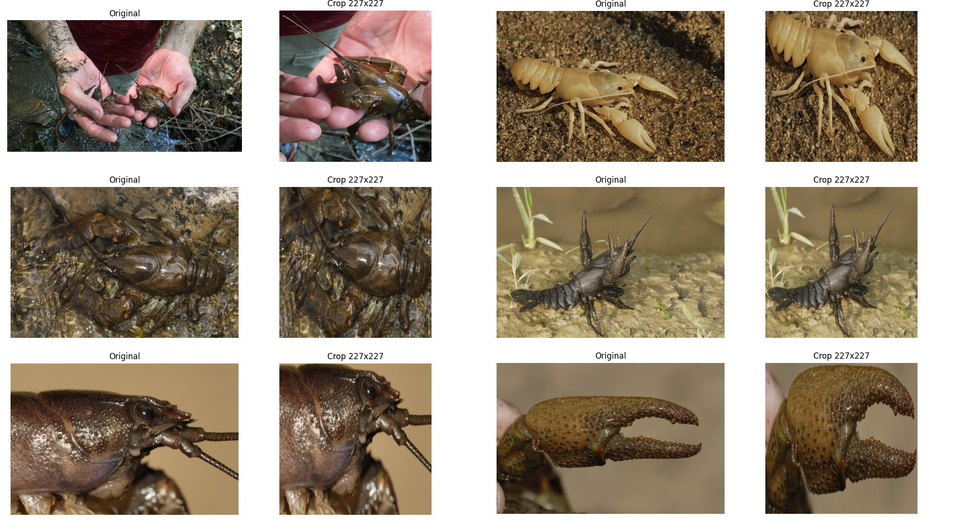
\includegraphics[width=\textwidth]{figs/torrentium_grid.png}
    \caption{Exemple din setul de date procesat pentru specia
    \textit{Austropotamobius torrentium}: imaginea originală (stânga)
    și regiunea de interes extrasă la rezoluția 227×227 pixeli (dreapta),
    pentru șase specimene reprezentative.}
    \label{fig:crop_torrentium}
\end{figure}
\begin{figure}[!htb]
    \centering
    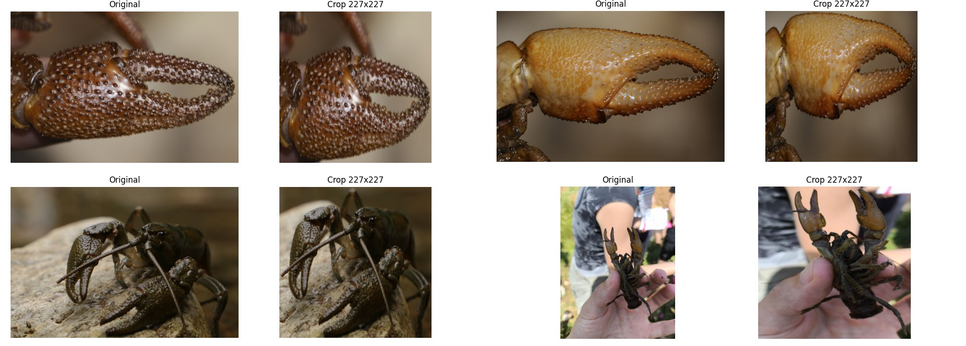
\includegraphics[width=\textwidth]{figs/bihariensis_grid.png}
    \caption{Exemple din setul de date procesat pentru specia
    \textit{Austropotamobius bihariensis}: imaginea originală (stânga)
    și regiunea de interes extrasă la rezoluția 227×227 pixeli (dreapta),
    pentru patru specimene reprezentative.}
    \label{fig:crop_bihariensis}
\end{figure}
\newpage


\section{Arhitectura modelului și transfer learning}

AlexNet \cite{krizhevsky2012imagenet} este o rețea neuronală convoluțională profundă compusă din cinci straturi convoluționale urmate de trei straturi complet conectate, proiectată inițial pentru clasificarea imaginilor din setul de date ImageNet pe 1000 de clase. În acest studiu, arhitectura este adaptată pentru clasificarea binară a celor două specii de rac, \textit{Austropotamobius bihariensis} și \textit{Austropotamobius torrentium}, prin tehnica transfer learning.




\subsection{Arhitectura AlexNet}

Imaginea de intrare are dimensiunea 227×227×3 pixeli. Deși  lucrarea originală \cite{krizhevsky2012imagenet} menționează o dimensiune de intrare de 224×224 pixeli, valoarea corectă din punct de vedere matematic, confirmată de dimensiunile hărților de caracteristici raportate în aceeași lucrare și utilizată în implementările moderne ale arhitecturii \cite{suh2018alexnet}, este de 227×227 pixeli. În consecință, toate imaginile din setul de date au fost redimensionate la 227×227 pixeli în etapa de preprocesare. Structura detaliată a arhitecturii este prezentată în Tabelul~\ref{tab:alexnet}.

\begin{table}[H]
\centering
\caption{Structura detaliată a arhitecturii AlexNet
\cite{krizhevsky2012imagenet}.}
\label{tab:alexnet}
\begin{tabular}{llcccc}
\hline
\textbf{Strat} & \textbf{Tip} & \textbf{Dimensiune ieșire} &
\textbf{Kernel} & \textbf{Pas} & \textbf{Activare} \\
\hline
Input   & Imagine      & 227×227×3   & --    & -- & --      \\
\hline
1       & Convoluție   & 55×55×96    & 11×11 & 4  & ReLU    \\
        & Max Pooling  & 27×27×96    & 3×3   & 2  & --      \\
\hline
2       & Convoluție   & 27×27×256   & 5×5   & 1  & ReLU    \\
        & Max Pooling  & 13×13×256   & 3×3   & 2  & --      \\
\hline
3       & Convoluție   & 13×13×384   & 3×3   & 1  & ReLU    \\
\hline
4       & Convoluție   & 13×13×384   & 3×3   & 1  & ReLU    \\
\hline
5       & Convoluție   & 13×13×256   & 3×3   & 1  & ReLU    \\
        & Max Pooling  & 6×6×256     & 3×3   & 2  & --      \\
\hline
6       & FC           & 4096        & --    & -- & ReLU    \\
7       & FC           & 4096        & --    & -- & ReLU    \\
8       & FC           & 1000        & --    & -- & Softmax \\
\hline
\end{tabular}
\end{table}





\subsection{Adaptarea prin transfer learning}

Ponderile straturilor convoluționale ale modelului AlexNet sunt inițializate cu valorile pre-antrenate pe setul de date ImageNet, care conține 1.2 milioane de imagini din 1000 de categorii vizuale diverse \cite{krizhevsky2012imagenet}. Aceste ponderi sunt menținute înghețate pe parcursul antrenării, adică nu sunt actualizate prin propagare inversă. Justificarea acestei alegeri constă în faptul că straturile convoluționale ale unui model pre-antrenat pe ImageNet învață reprezentări vizuale generale (muchii, texturi, forme) transferabile la domenii noi față de ImageNet, inclusiv la imaginile din domeniul biologiei acvatice.

Adaptarea modelului la problema de față constă în două intervenții. În primul rând, blocul convoluțional (\texttt{features}), compus din cele cinci straturi convoluționale și operațiile de max-pooling asociate, este înghețat: ponderile sale pre-antrenate pe ImageNet sunt menținute fixe pe parcursul întregului proces de antrenare și nu sunt actualizate prin propagare inversă. În al doilea rând, stratul de ieșire original (stratul FC 8), proiectat pentru 1000 de clase, este înlocuit cu un nou strat complet conectat cu 2 neuroni de ieșire, corespunzând celor două specii clasificate: \textit{Austropotamobius bihariensis} și \textit{Austropotamobius torrentium}. Straturile complet conectate FC 6 și FC 7, cu ponderile lor inițializate din ImageNet, sunt păstrate și ajustate (\textit{fine-tuned}) împreună cu noul strat de ieșire pe parcursul antrenării. În total, din cei 57.012.034 de parametri ai modelului, 2.469.696 (4,3\%) aparțin blocului convoluțional și rămân înghețați, iar 54.542.338 (95,7\%) sunt antrenabili, reprezentând întregul bloc al clasificatorului FC. Structura modificată este prezentată în Tabelul~\ref{tab:alexnet_adaptat}.

Dimensiunea straturilor FC 6 și FC 7 (4096 de neuroni fiecare) a fost păstrată identică cu arhitectura originală, deși acest nivel ascuns este neobișnuit de mare în raport cu dimensiunea redusă a stratului de ieșire (2 neuroni). Opțiunea a fost motivată de dorința de a exploata cât mai eficient ponderile pre-antrenate pe ImageNet ale acestor straturi. Pentru a evalua această decizie, a fost testată și o variantă alternativă a clasificatorului, cu un strat ascuns redus la 512 de neuroni (9216$\rightarrow$512$\rightarrow$2), inițializat aleatoriu și antrenat de la zero, fără a beneficia de ponderile pre-antrenate ale straturilor FC originale. Această variantă a obținut o acuratețe pe setul de testare de 91,84\%, inferioară configurației cu clasificator complet (4096 de neuroni, 95,92\%), confirmând că păstrarea dimensiunii originale a straturilor FC permite o valorificare mai eficientă a reprezentărilor învățate pe ImageNet, comparativ cu un clasificator mai mic, antrenat de la zero. Structura modificată a clasificatorului final este prezentată în Tabelul~\ref{tab:alexnet_adaptat}.

\begin{table}[H]
\centering
\caption{Structura AlexNet adaptată prin transfer learning pentru
clasificarea binară a speciilor de \textit{Austropotamobius}.}
\label{tab:alexnet_adaptat}
\begin{tabular}{llccc}
\hline
\textbf{Strat} & \textbf{Tip} & \textbf{Dimensiune ieșire} &
\textbf{Ponderi inițiale} & \textbf{Antrenat} \\
\hline
Input   & Imagine      & 227×227×3   & --           & --          \\
\hline
1       & Convoluție   & 55×55×96    & ImageNet     & Nu          \\
        & Max Pooling  & 27×27×96    & --           & --          \\
\hline
2       & Convoluție   & 27×27×256   & ImageNet     & Nu          \\
        & Max Pooling  & 13×13×256   & --           & --          \\
\hline
3       & Convoluție   & 13×13×384   & ImageNet     & Nu          \\
\hline
4       & Convoluție   & 13×13×384   & ImageNet     & Nu          \\
\hline
5       & Convoluție   & 13×13×256   & ImageNet     & Nu          \\
        & Max Pooling  & 6×6×256     & --           & --          \\
\hline
6       & FC           & 4096        & ImageNet     & \textbf{Da} \\
7       & FC           & 4096        & ImageNet     & \textbf{Da} \\
\hline
8       & FC           & 2           & Inițializare & \textbf{Da} \\
        &              &             & aleatorie    &             \\
\hline
\end{tabular}
\end{table}

Această abordare permite obținerea unor performanțe ridicate chiar și în condiții de eșantionare limitată, compensând dimensiunea redusă a setului de date disponibil (318 imagini) față de cerințele tipice ale antrenării de la zero a unei rețele convoluționale profunde \cite{krizhevsky2012imagenet}.






\section{Antrenarea modelului}\label{sec:antrenare}

\subsection{Împărțirea setului de date}

Setul de date procesat, conținând 318 imagini, este împărțit în trei subseturi disjuncte: antrenare, validare și testare. Împărțirea este realizată stratificat, separat pentru fiecare clasă, pentru a menține proporțiile originale ale distribuției în toate cele trei subseturi. Rapoartele utilizate sunt 70\% pentru antrenare, 15\% pentru validare și 15\% pentru testare, rezultând distribuția prezentată în Tabelul~\ref{tab:split}.

\begin{table}[H]
\centering
\caption{Distribuția imaginilor pe subseturi de antrenare, validareși testare.}
\label{tab:split}
\begin{tabular}{lcccc}
\hline
\textbf{Specie} & \textbf{Total} & \textbf{Antrenare} &
\textbf{Validare} & \textbf{Testare} \\
\hline
\textit{A. bihariensis} & 182 & 127 & 27 & 28 \\
\textit{A. torrentium}  & 136 & 95  & 20 & 21 \\
\hline
\textbf{Total}          & 318 & 222 & 47 & 49 \\
\hline
\end{tabular}
\end{table}

Reproductibilitatea împărțirii este asigurată prin fixarea unei semințe aleatoare (\textit{random seed}) cu valoarea 42, aplicată consistent pentru generatoarele de numere aleatoare din bibliotecile Python, NumPy și PyTorch.

\subsection{Augmentarea datelor de antrenare}

Datorită dimensiunii reduse a setului de antrenare (222 de imagini), este aplicat un set extins de tehnici de augmentare la runtime, exclusiv pe datele de antrenare. Seturile de validare și testare nu sunt supuse augmentării, conținând doar imaginile originale preprocesate, pentru a asigura o evaluare obiectivă a performanței modelului. Tehnicile de augmentare aplicate sunt prezentate în Tabelul~\ref{tab:augmentare}.

\begin{table}[H]
\centering
\caption{Tehnicile de augmentare aplicate la runtime pe setul de antrenare.}
\label{tab:augmentare}
\begin{tabular}{lp{7cm}}
\hline
\textbf{Tehnică} & \textbf{Parametri} \\
\hline
Oglindire orizontală    & Probabilitate 0.5 \\
Oglindire verticală     & Probabilitate 0.3 \\
Rotație aleatorie       & Unghi maxim ±45° \\
Deformare perspectivă   & Scală distorsiune 0.3, probabilitate 0.4 \\
Crop aleatoriu          & Scală 80--100\%, raport aspect 0.9--1.1 \\
Variație culoare        & Luminozitate 0.4, contrast 0.4,
                          saturație 0.3, nuanță 0.1 \\
Conversie tonuri de gri & Probabilitate 0.1 \\
Blur gaussian           & Kernel 3×3, $\sigma \in [0{.}1,\ 2{.}0]$ \\
Ștergere aleatorie      & Probabilitate 0.3, scală 2--15\%
                          din suprafața imaginii \\
\hline
\end{tabular}
\end{table}

Figura~\ref{fig:augmentari_bihariensis} și Figura~\ref{fig:augmentari_torrentium} ilustrează imaginea originală și opt variante augmentate ale aceleiași imagini, pentru câte un specimen din fiecare specie, generate prin aplicarea succesivă a tehnicilor prezentate în Tabelul~\ref{tab:augmentare}. Deasupra fiecărei variante sunt indicate tehnicile activate efectiv la acea rulare, dat fiind caracterul stocastic al augmentării (fiecare tehnică se activează independent, pe baza probabilității proprii).

\begin{figure}[htbp]
    \centering
    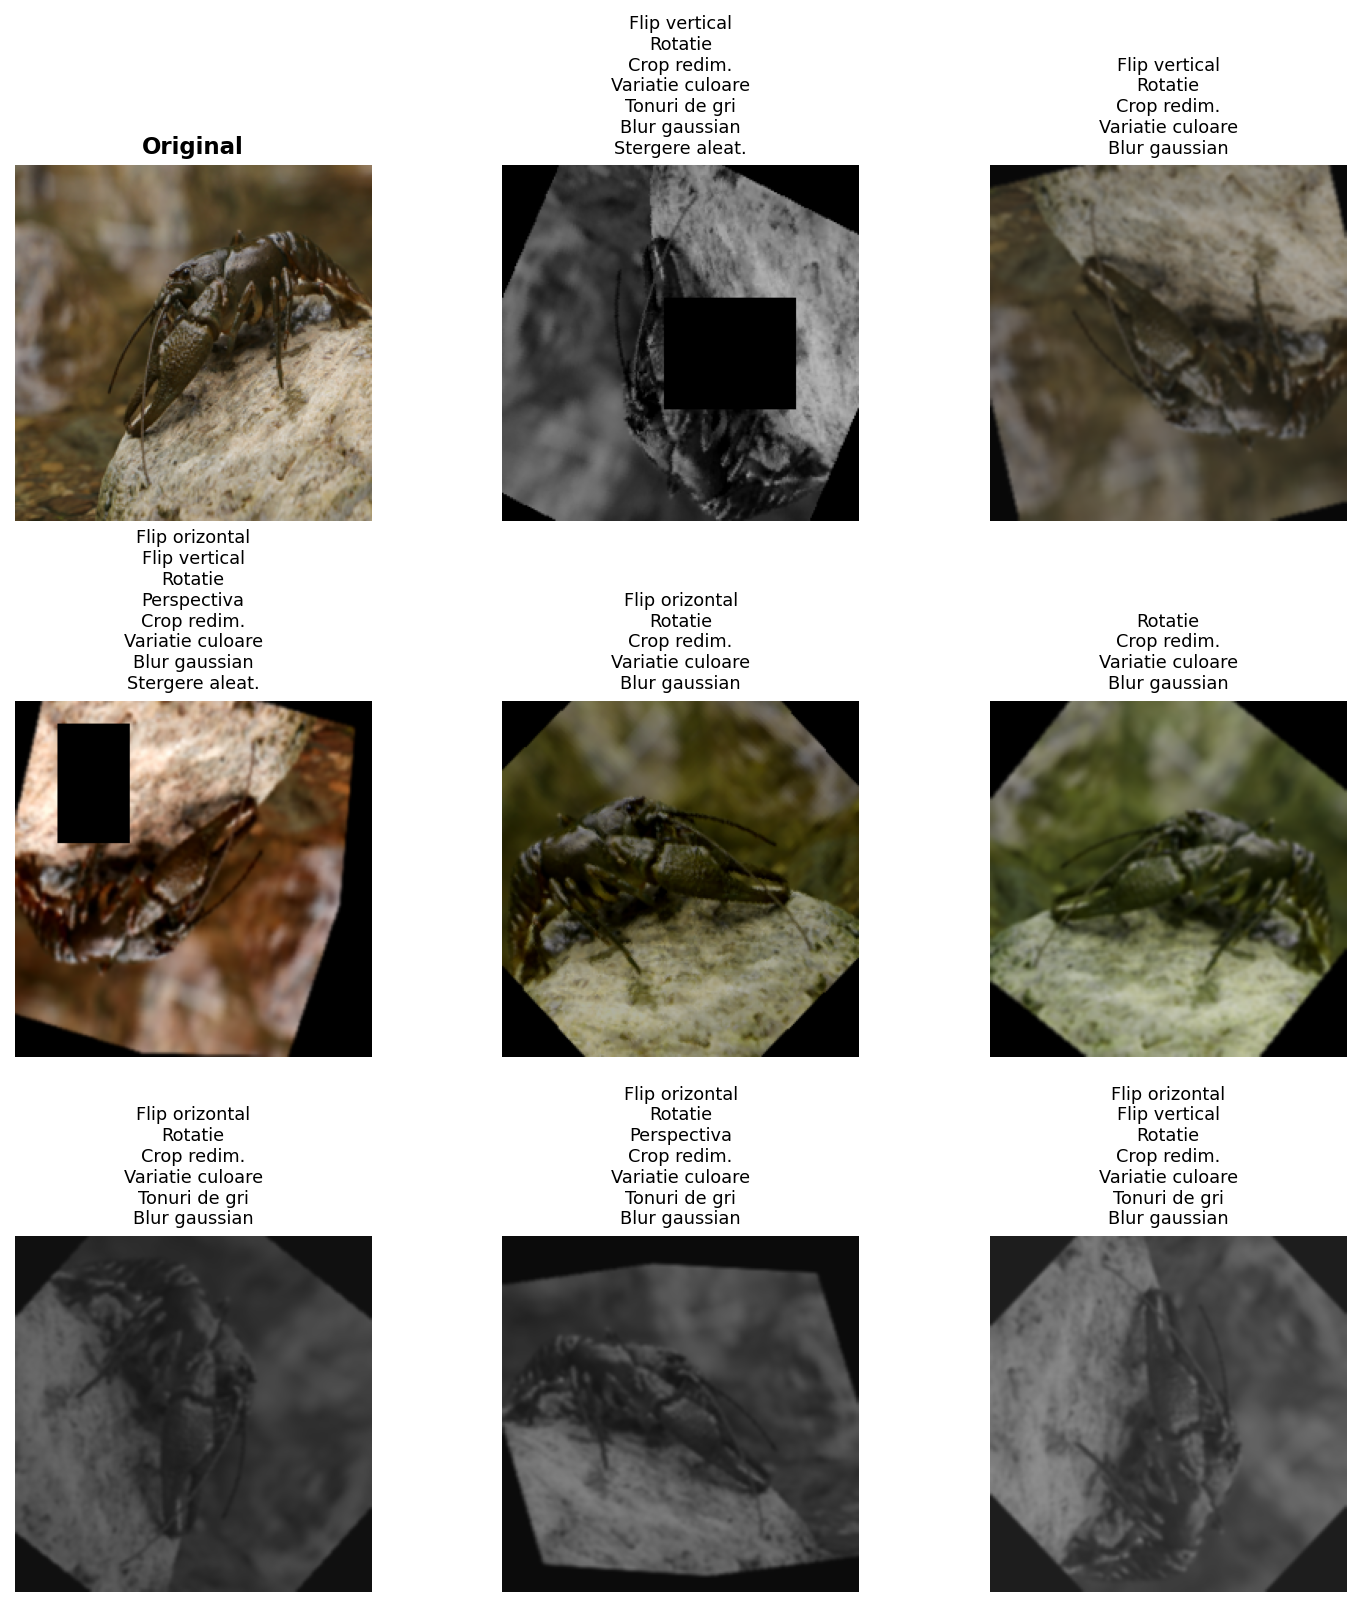
\includegraphics[width=\textwidth]{figs/AugmentariGridBihariensis.png}
    \caption{Imaginea originală și opt variante augmentate ale unui
    specimen de \textit{Austropotamobius bihariensis}, cu tehnicile
    aplicate la fiecare rulare indicate deasupra imaginii
    corespunzătoare.}
    \label{fig:augmentari_bihariensis}
\end{figure}

\begin{figure}[htbp]
    \centering
    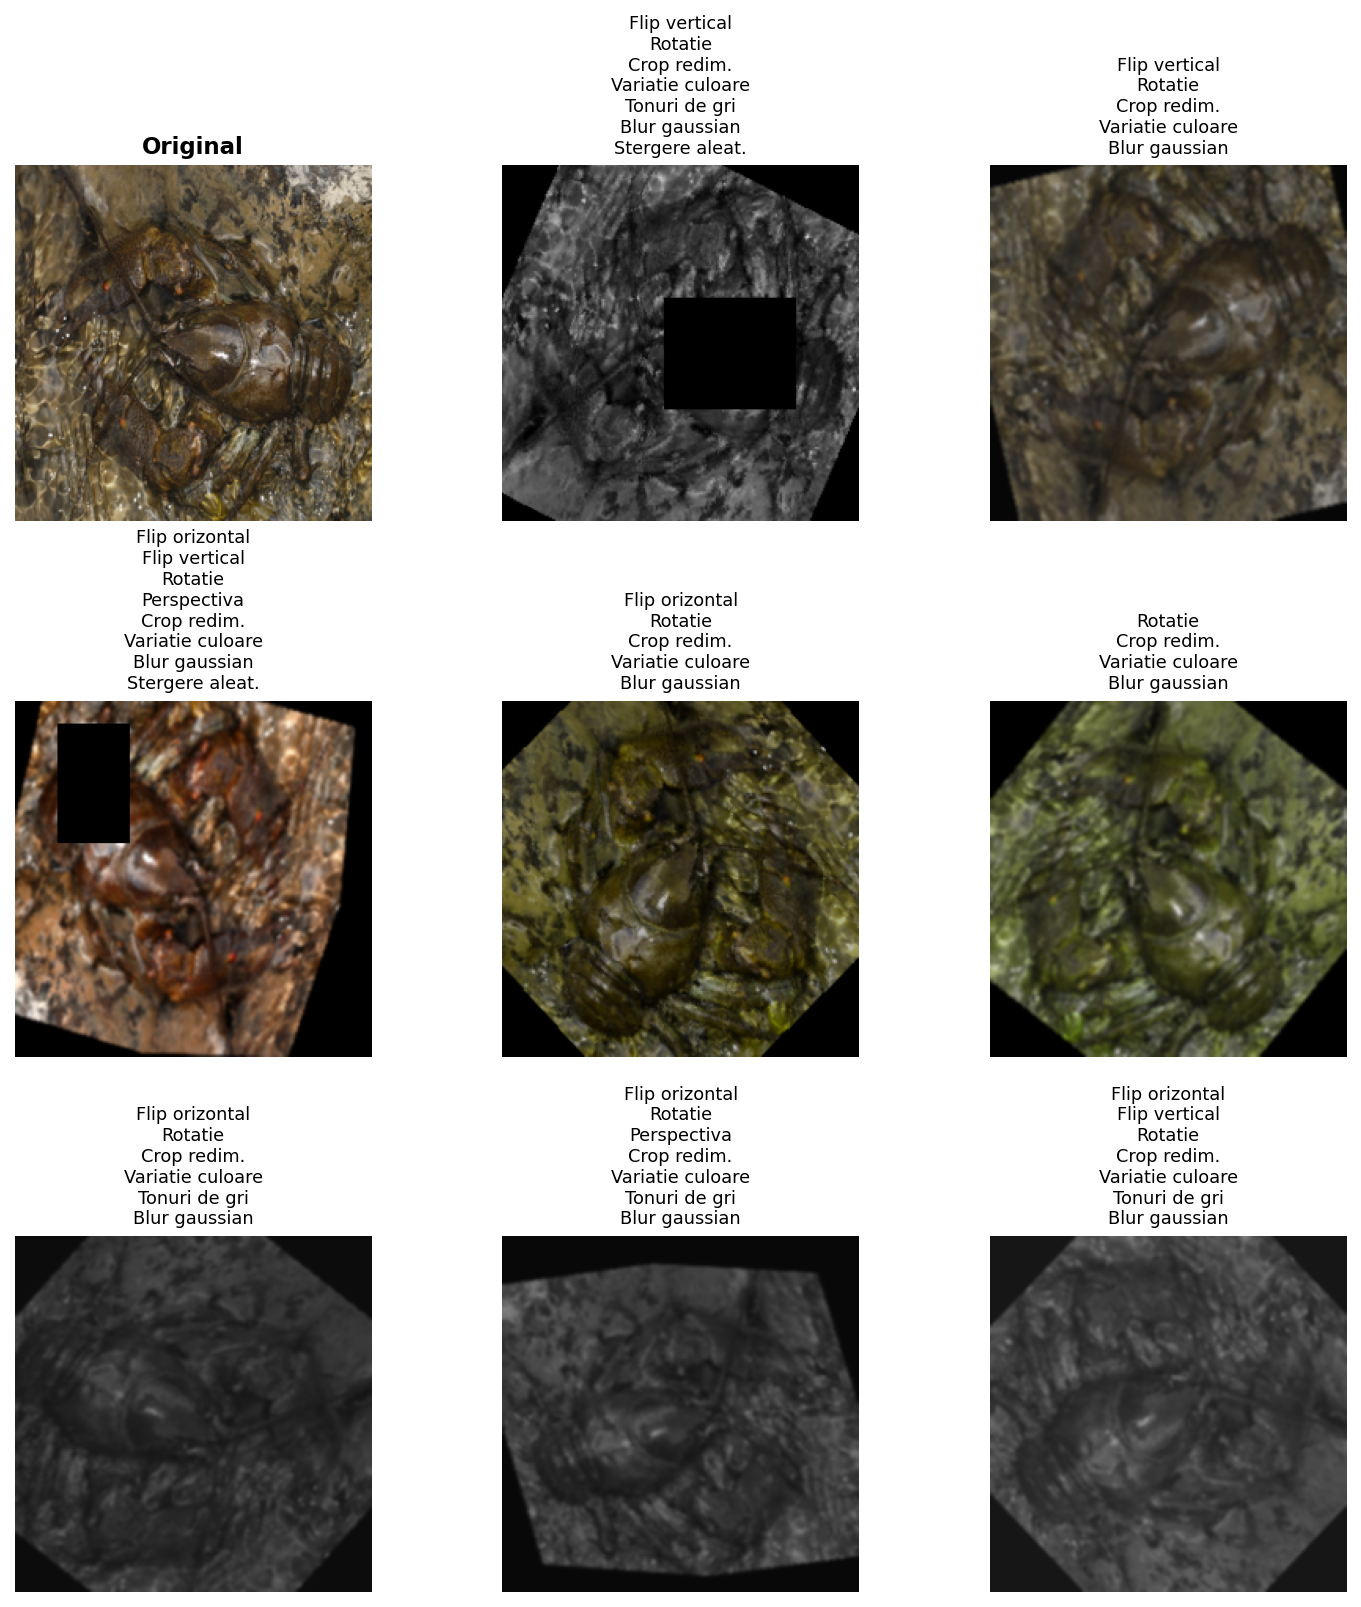
\includegraphics[width=\textwidth]{figs/AugmentariGridTorrentium.png}
    \caption{Imaginea originală și opt variante augmentate ale unui
    specimen de \textit{Austropotamobius torrentium}, cu tehnicile
    aplicate la fiecare rulare indicate deasupra imaginii
    corespunzătoare.}
    \label{fig:augmentari_torrentium}
\end{figure}



\subsection{Normalizarea datelor}

Toate imaginile, indiferent de subset, sunt normalizate cu media și deviația standard calculate pe setul de date ImageNet: $\mu = [0{,}485,\ 0{,}456,\ 0{,}406]$ și $\sigma = [0{,}229,\ 0{,}224,\ 0{,}225]$, care corespund canalelor RGB. Această normalizare este necesară pentru compatibilitatea cu ponderile pre-antrenate ale modelului AlexNet, care au fost obținute pe date procesate cu aceleași constante \cite{krizhevsky2012imagenet}.

\subsection{Configurația antrenării}

Antrenarea este realizată pe 60 de epoci cu un batch size de 32 de imagini. Funcția de pierdere utilizată este Cross-Entropy Loss cu Label Smoothing de 0.1, aplicat pentru a reduce supra-încrederea modelului  în predicțiile sale (\textit{overconfidence}) și a îmbunătăți generalizarea pe seturi de date mici.

Optimizatorul utilizat este SGD (\textit{Stochastic Gradient Descent}) cu coeficient pentru termenul momentum egal cu 0.9, rată de învățare inițială 0.001 și weight decay 0,0005. Rata de învățare este ajustată automat printr-un planificator (\textit{scheduler}) de tip \textit{ReduceLROnPlateau}, care reduce rata de învățare cu un factor de 0.1 atunci când pierderea pe setul de validare nu se îmbunătățește timp de 10 epoci consecutive.

Selecția modelului final se face pe baza celei mai bune valori a acurateții obținute pe setul de validare pe parcursul antrenării, ponderile corespunzătoare fiind salvate și utilizate ulterior pentru evaluarea pe setul de testare. Configurația completă a hiperparametrilor este prezentată în Tabelul~\ref{tab:hiperparametri}.

\begin{table}[H]
\centering
\caption{Configurația hiperparametrilor utilizați în antrenare.}
\label{tab:hiperparametri}
\begin{tabular}{lc}
\hline
\textbf{Hiperparametru} & \textbf{Valoare} \\
\hline
Număr epoci          & 60 \\
Batch size           & 32 \\
Rată de învățare     & 0.001 \\
Momentum             & 0.9 \\
Weight decay         & 0.0005 \\
Label smoothing      & 0.1 \\
Optimizer            & SGD \\
Scheduler            & ReduceLROnPlateau \\
Factor reducere LR   & 0.1 \\
Răbdare scheduler    & 10 epoci \\
Random seed          & 42 \\
\hline
\end{tabular}
\end{table}








\section{Evaluarea performanței}

Performanța modelului a fost evaluată pe setul de testare, format din 49 de imagini nevăzute de model în timpul antrenării (28 de specimene de \textit{Austropotamobius bihariensis} și 21 de specimene de \textit{Austropotamobius torrentium}). Metrica principală utilizată este acuratețea pe setul de testare, calculată ca raport între numărul de predicții corecte și numărul total de exemple din setul de test.

Pentru o evaluare mai detaliată a performanței pe fiecare clasă, au fost calculate suplimentar metricile precizie (\textit{precision}), rata de regăsire (\textit{recall}) și scorul F1 (\textit{F1-score}), pe baza matricei de confuzie prezentate în Tabelul~\ref{tab:confuzie}.

\begin{table}[H]
\centering
\caption{Matricea de confuzie pe setul de testare.}
\label{tab:confuzie}
\begin{tabular}{lcc}
\hline
\textbf{Specia reală} & \textbf{Prezis \textit{bihariensis}} & \textbf{Prezis \textit{torrentium}} \\
\hline
\textit{A. bihariensis} & 27 & 1 \\
\textit{A. torrentium}  & 1  & 20 \\
\hline
\end{tabular}
\end{table}

Tabelul~\ref{tab:metrici} prezintă precizia, rata de regăsire și scorul F1 calculate pentru fiecare clasă în parte.

\begin{table}[H]
\centering
\caption{Precizia, rata de regăsire și scorul F1 pe fiecare clasă.}
\label{tab:metrici}
\begin{tabular}{lccc}
\hline
\textbf{Specia} & \textbf{Precizie} & \textbf{Recall} & \textbf{F1-score} \\
\hline
\textit{A. bihariensis} & 0.9643 & 0.9643 & 0.9643 \\
\textit{A. torrentium}  & 0.9524 & 0.9524 & 0.9524 \\
\hline
\end{tabular}
\end{table}

Valorile apropiate ale celor trei metrici pentru ambele clase confirmă un comportament echilibrat al modelului, fără o tendință sistematică de a favoriza o specie în detrimentul celeilalte. Scorul F1 mediu (macro-mediu) obținut este de 0,9583.

Modelul final a fost obținut printr-un proces iterativ de rafinare, în care fiecare etapă a adus îmbunătățiri măsurabile față de configurația anterioară. Evoluția acurateții pe setul de testare de-a lungul celor patru configurații experimentate este prezentată în Tabelul~\ref{tab:evolutie_runs}.

\begin{table}[H]
\centering
\caption{Evoluția acurateții pe setul de testare în funcție de
configurația experimentată.}
\label{tab:evolutie_runs}
\begin{tabular}{cp{9cm}c}
\hline
\textbf{Configurație} & \textbf{Modificări față de configurația anterioară}
& \textbf{Acuratețe test} \\
\hline
1 & Split stratificat 70/15/15, fără alte intervenții & 62.50\% \\
2 & + Înghețare convoluții, normalizare ImageNet, augmentări, seed fix & 87.50\% \\
3 & + Extragere regiuni de interes (crop cu LabelMe) & \textbf{95.92\%} \\
4 & Identic cu configurația 3, batch size 64 & 93.88\% \\
\hline
\end{tabular}
\end{table}

Prima configurație, folosind exclusiv împărțirea stratificată a datelor fără nicio altă intervenție, a produs o acuratețe de 62,50\% pe setul de testare, cu puțin peste nivelul unei clasificări aleatorii binare, indicând că modelul nu reușea să extragă trăsături discriminante relevante din imaginile brute neadnotate.

Introducerea în celei de-a doua configurații a înghețării blocului convoluțional, a normalizării ImageNet, a augmentărilor la runtime și a fixării semințelor aleatoare a adus un salt semnificativ la 87,50\%, confirmând că transferul de cunoștințe din ImageNet este eficient chiar și pe un set de date de dimensiune redusă, cu condiția ca datele de intrare să fie compatibile cu formatul așteptat de model.

Cel mai important salt de performanță a fost produs de introducerea extragerii automate a regiunilor de interes pe baza adnotărilor LabelMe. Prin eliminarea fondului irelevant (substrat acvatic, vegetație, mâini ale colectorului) și centrarea imaginii pe specimenul de interes, modelul a avut acces la trăsăturile morfologice discriminante ale celor două specii, ceea ce a condus la o acuratețe de 95,92\% în cea de-a treia configurație. Extragerea regiunilor de interes a fost aplicată uniform pe toate cele trei subseturi (antrenare, validare și testare), înainte de împărțirea stratificată a datelor, astfel încât evaluarea pe setul de testare să reflecte fidel performanța modelului pe imagini deja procesate prin același flux.

Creșterea dimensiunii batch-ului la 64 în cea de-a patra configurație a dus la o ușoară scădere a acurateței la 93,88\%, sugerând că un batch size mai mic favorizează generalizarea în contextul unui set de antrenare de dimensiuni reduse (222 de imagini). Modelul reținut ca rezultat final al lucrării corespunde configurației 3, cu o acuratețe pe setul de testare de \textbf{95,92\%}.


% detalii privind construirea setului de date


\chapter{Rezultate și discuții} \label{chapter:cap5} 

Acest capitol prezintă rezultatele experimentale obținute de modelul final, descris în Capitolul~\ref{chapter:cap4}, și discută semnificația acestora. Sunt prezentate, în primul rând, performanța globală a modelului pe setul de testare independent și exemple individuale de clasificare, ilustrând comportamentul acestuia pe specimene cu grade variate de încredere. Este analizată, în continuare, evoluția acurateții de-a lungul celor patru configurații experimentate, evidențiind contribuția fiecărei intervenții tehnice asupra performanței finale. Capitolul se închide cu o comparație între rezultatele obținute și abordările existente din literatură, discutate în Capitolul~\ref{chapter:cap3}.


\section{Rezultate experimentale}

Modelul final, obținut prin adaptarea arhitecturii AlexNet cu transfer learning din ImageNet și antrenat pe un set de 222 de imagini, a fost evaluat pe un set de testare independent format din 49 de imagini (28 de specimene de \textit{Austropotamobius bihariensis} și 21 de specimene de \textit{Austropotamobius torrentium}). Acuratețea obținută pe setul de testare este de \textbf{95,92\%}, corespunzând unui număr de 47 de predicții corecte din 49.

Rezultatul a fost obținut în configurația 3, care introduce extragerea automată a regiunilor de interes pe baza adnotărilor LabelMe, cu un batch size de 32 de imagini, înghețarea blocului convoluțional, normalizare ImageNet și augmentări la runtime. Selecția modelului salvat s-a realizat pe baza celei mai bune acurateți pe setul de validare, obținută în cursul celor 60 de epoci de antrenare.

Pentru a ilustra comportamentul modelului pe imagini individuale, Figura~\ref{fig:pred1}--Figura~\ref{fig:pred5} prezintă exemple reprezentative de clasificare, selectate din setul de testare utilizat la evaluarea oficială a modelului, incluzând atât predicții corecte cu grade variate de încredere, cât și cazul de clasificare incorectă identificat în Tabelul~\ref{tab:confuzie}.

\begin{figure}[H]
    \centering
    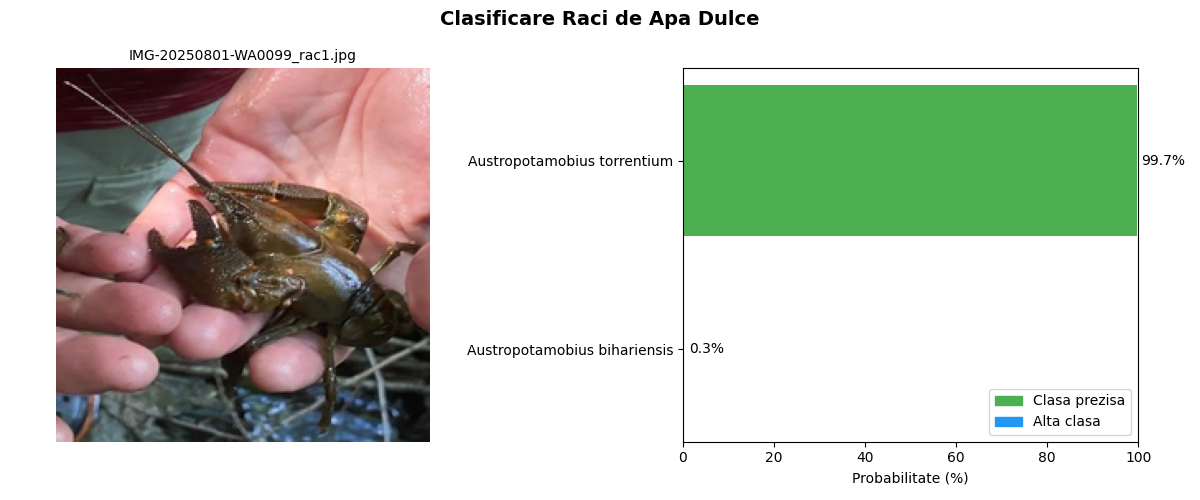
\includegraphics[width=\textwidth]{figs/Pred1_FoarteMare_Torrentium.png}
    \caption{Clasificare corectă cu încredere foarte ridicată:
    specimen de \textit{Austropotamobius torrentium} identificat
    corect cu probabilitatea de 99,7\%.}
    \label{fig:pred1}
\end{figure}

\begin{figure}[H]
    \centering
    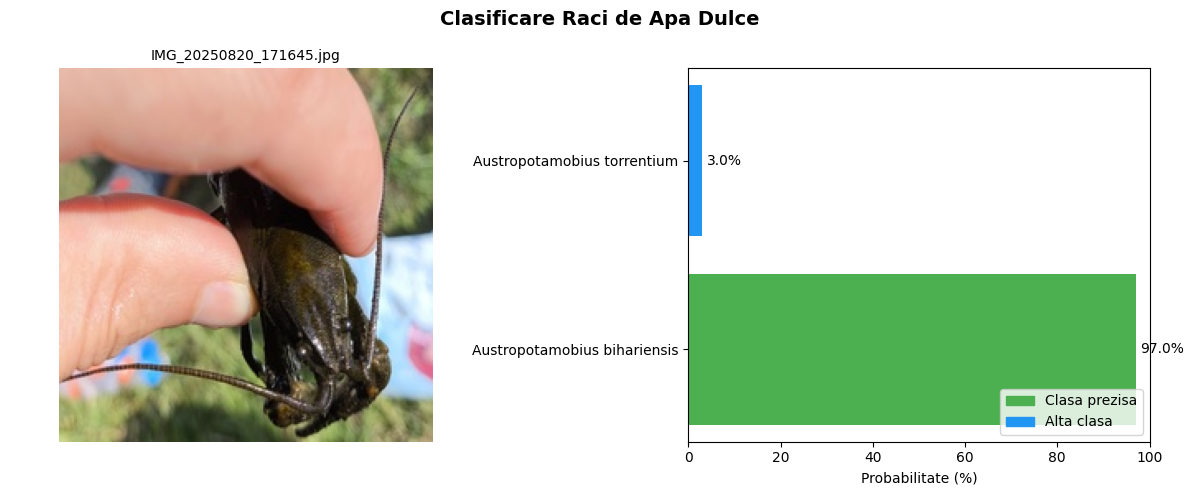
\includegraphics[width=\textwidth]{figs/Pred2_Mare_Bihariensis.png}
    \caption{Clasificare corectă cu încredere ridicată: specimen
    de \textit{Austropotamobius bihariensis} identificat corect
    cu probabilitatea de 97,0\%.}
    \label{fig:pred2}
\end{figure}

\begin{figure}[H]
    \centering
    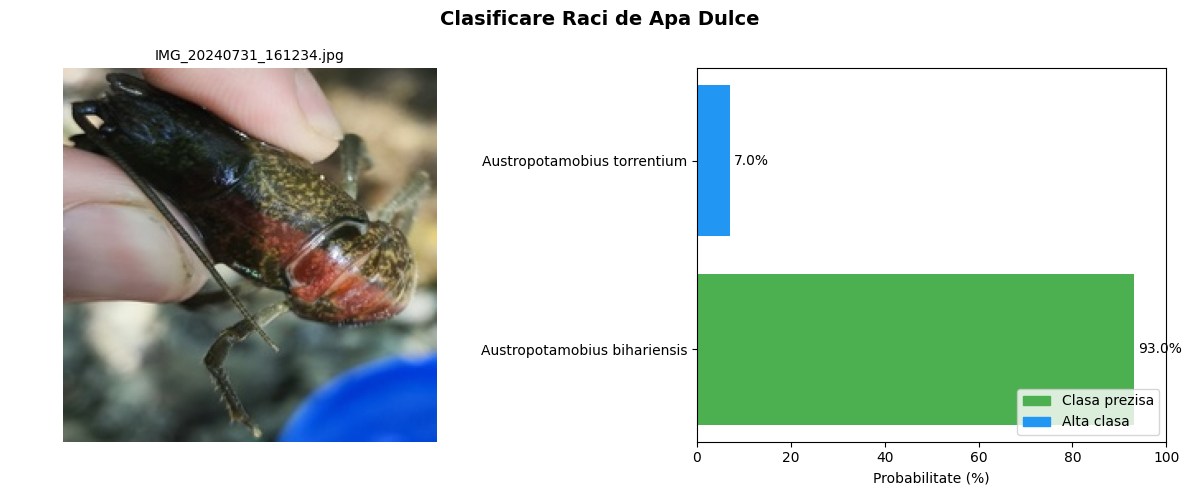
\includegraphics[width=\textwidth]{figs/Pred3_Moderata_Bihariensis.png}
    \caption{Clasificare corectă cu încredere moderată: specimen
    de \textit{Austropotamobius bihariensis} identificat corect
    cu probabilitatea de 93,0\%.}
    \label{fig:pred3}
\end{figure}

\begin{figure}[H]
    \centering
    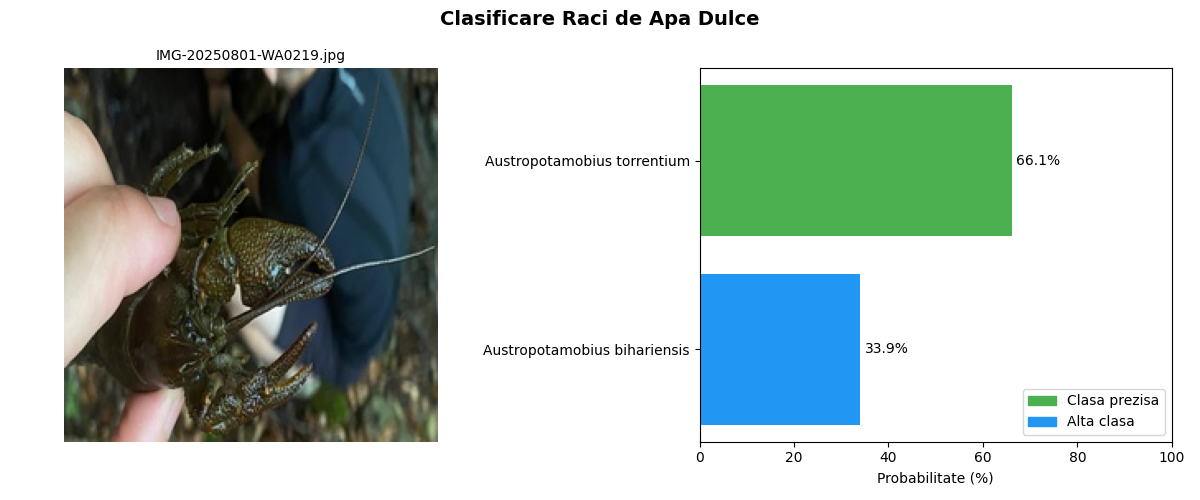
\includegraphics[width=\textwidth]{figs/Pred4_Mica_Torrentium.png}
    \caption{Clasificare corectă cu încredere scăzută: specimen
    de \textit{Austropotamobius torrentium} identificat corect
    cu probabilitatea de 66,1\%.}
    \label{fig:pred4}
\end{figure}

\begin{figure}[H]
    \centering
    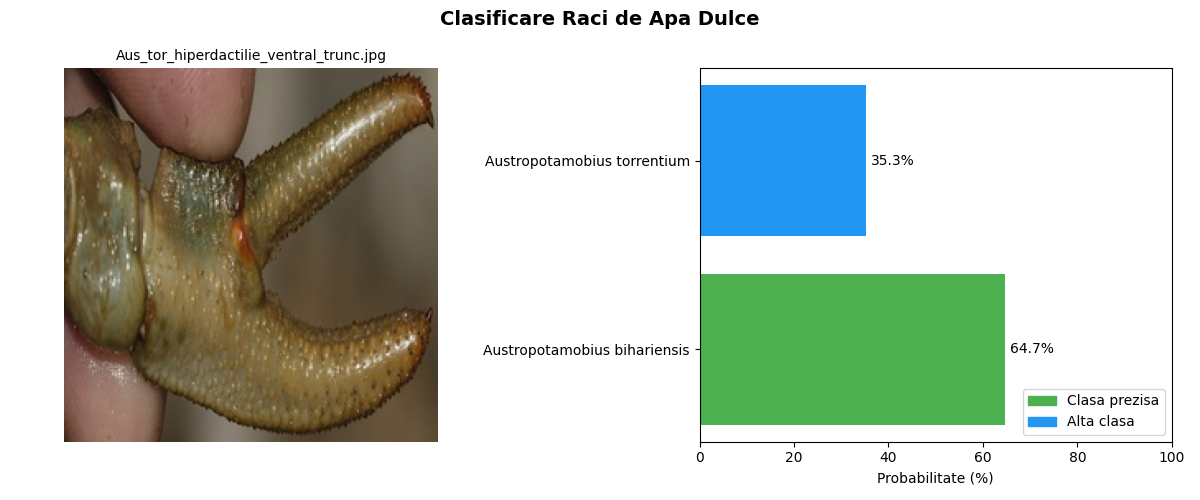
\includegraphics[width=\textwidth]{figs/Pred5_Gresit_Torrentium_ca_Bihariensis.png}
    \caption{Clasificare incorectă: specimen de \textit{Austropotamobius
    torrentium} clasificat eronat ca \textit{Austropotamobius bihariensis}
    cu probabilitatea de 64,7\%.}
    \label{fig:pred5}
\end{figure}

\section{Analiza rezultatelor}

Acuratețea de 95,92\% obținută pe setul de testare demonstrează că arhitectura AlexNet cu transfer learning este capabilă să discrimineze eficient între cele două specii de \textit{Austropotamobius} chiar și în condiții de eșantionare limitată. Evoluția performanței de-a lungul celor patru configurații experimentate relevă contribuția distinctă a fiecărei intervenții tehnice.

Primul salt major de performanță, de la 62,50\% la 87,50\%, a fost produs de introducerea înghețării blocului convoluțional, a normalizării ImageNet și a augmentărilor la runtime. Această îmbunătățire confirmă că reprezentările vizuale generale învățate de AlexNet pe ImageNet sunt suficient de expresive pentru a descrie morfologia racilor de apă dulce, fără a necesita reantrenarea convoluțiilor de la zero.

Al doilea salt major, de la 87,50\% la 95,92\%, a fost determinat de introducerea extragerii regiunilor de interes pe baza adnotărilor manuale realizate în LabelMe, urmate de decuparea automată a acestora, conform fluxului descris în Secțiunea~\ref{chapter:cap4}. Procesul nu a implicat un model de detecție automată (precum YOLO) pentru localizarea specimenelor: bounding box-urile au fost trasate manual pentru fiecare imagine, automatizarea limitându-se la etapele de decupare, redimensionare și organizare a imaginilor rezultate.

Scăderea acurateței de la 95,92\% la 93,88\% la creșterea batch size-ului de la 32 la 64 sugerează că, în contextul unui set de antrenare de dimensiuni reduse (222 de imagini), un batch size mai mic produce estimări ale gradientului mai zgomotoase dar mai reprezentative, favorizând generalizarea modelului.

\section{Comparație cu metode existente}

Lucrările prezentate în capitolul~\ref{chapter:cap3} abordează problema identificării racilor de apă dulce prin tehnici de detecție și segmentare de obiecte (YOLOv11n, YOLOv8n), pe seturi de date considerabil mai mari și pe specii diferite față de cele vizate aici. Prin natura lor, aceste metode rezolvă o problemă distinctă față de clasificarea binară propusă aici: ele localizează și delimitează specimenele în imagini de teren neprelucrate, în timp ce modelul dezvoltat în această lucrare clasifică imagini deja centrate pe specimen.

Diferența fundamentală de task (detecție și segmentare față de clasificare binară), de specii vizate și de dimensiunea seturilor de date utilizate face imposibilă o comparație numerică directă a performanțelor. Cu toate acestea, acuratețea de 95,92\% obținută pe un set de testare independent, în condițiile unui set de antrenare de doar 222 de imagini, demonstrează că abordarea prin transfer learning reprezintă o soluție viabilă pentru identificarea automată a speciilor din genul \textit{Austropotamobius} în condiții de eșantionare limitată, situație frecventă în studiile de biodiversitate pe specii protejate.



% \section{Rezultate experimentale}
% \section{Analiza rezultatelor}
% \section{Comparație cu metode existente}

\chapter{Concluzii}\label{chapter:cap6}

Acest capitol sintetizează concluziile finale ale lucrării pe baza rezultatelor prezentate în Capitolul~\ref{chapter:cap5}, evidențiază principalele limitări ale abordării propuse și prezintă direcțiile de dezvoltare ulterioară a soluției de clasificare automată a celor două specii de \textit{Austropotamobius}.


Lucrarea de față a demonstrat că identificarea automată a speciilor de raci de apă dulce din genul \textit{Austropotamobius} prin tehnici de deep learning reprezintă o abordare viabilă și eficientă chiar și în condiții de eșantionare limitată. Prin adaptarea arhitecturii AlexNet cu transfer learning din ImageNet și antrenarea pe un set de date de 318 imagini colectate din teren, s-a obținut o acuratețe de \textbf{95,92\%} pe setul de testare independent, demonstrând că modelul discriminează cu succes între \textit{Austropotamobius bihariensis} și \textit{Austropotamobius torrentium}.

Procesul iterativ de rafinare a evidențiat contribuția distinctă a fiecărei intervenții tehnice. Înghețarea blocului convoluțional și utilizarea reprezentărilor pre-antrenate pe ImageNet au produs primul salt major de performanță, de la 62,50\% la 87,50\%, confirmând transferabilitatea trăsăturilor vizuale generale la domeniul biologiei acvatice. Introducerea extragerii automate a regiunilor de interes pe baza adnotărilor LabelMe a generat al doilea salt semnificativ, de la 87,50\% la 95,92\%, subliniind importanța critică a calității datelor de intrare în raport cu complexitatea arhitecturii utilizate.

\section*{Limitări}

Principala limitare a lucrării constă în dimensiunea redusă a setului de date disponibil (318 imagini), care restrânge capacitatea de generalizare a modelului la variații morfologice și de iluminare nereprezentate în datele de antrenare. De asemenea, setul de date prezintă un dezechilibru moderat între clase (182 față de 136 de imagini), care, deși a fost gestionat prin împărțirea stratificată, poate influența performanța modelului pe clase subreprezentate. O altă limitare constă în necesitatea adnotării manuale prealabile a imaginilor pentru extragerea regiunilor de interes, ceea ce face ca fluxul actual să nu fie aplicabil direct pe imagini de teren neprelucrate fără intervenție umană.

\section*{Direcții viitoare}

Direcțiile de dezvoltare ulterioară vizează mai multe aspecte. Extinderea setului de date prin colectarea de noi imagini de teren ar permite antrenarea unor modele mai robuste și validarea performanței pe o varietate mai mare de condiții de captură. Înlocuirea arhitecturii AlexNet cu arhitecturi moderne de tip EfficientNet sau ResNet, proiectate pentru eficiență ridicată pe seturi de date mici, reprezintă o direcție naturală de îmbunătățire a performanței.

Integrarea unui modul de detecție automată a specimenelor direct pe imaginile de teren neprelucrate, prin tehnici de tip YOLO, ar elimina necesitatea adnotării manuale și ar permite construirea unui sistem complet automat de identificare a speciilor, utilizabil direct în activitățile de monitorizare a biodiversității acvatice. În final, extinderea clasificatorului la mai mult de două specii, prin includerea altor reprezentanți ai genului \textit{Austropotamobius} sau a altor specii de raci de apă dulce din România, ar crește semnificativ aplicabilitatea practică a sistemului dezvoltat.

% \chapter{Concluzii}

% \section{Concluzii finale}
% \section{Direcții viitoare}



\bibliography{mybib}
\bibliographystyle{alpha}
\addcontentsline{toc}{chapter}{Bibliography}

\appendix
\chapter{Anexă - Utilizarea instrumentelor de inteligență artificială generativă}
\label{genAIUsage}
În această anexă este prezentată o sinteză a modului în care au fost utilizate instrumentele de inteligență artificială generativă în cadrul lucrării. O imagine de ansamblu este oferită în Tabelul \ref{tab:genAIOverview}.

\begin{table}[h!]
    \centering
    \begin{tabularx}{\textwidth}{|l|X|X|X|}
            \hline \rowcolor{blue!20}
         Instrument AI& Scopul utilizării & Secțiuni în care a fost utilizat & Observații \\\hline
         \multirow{4}{*}{Claude Sonnet 4.6} & Traducerea abstractului din română în engleză & Abstract & Detalii în secțiunea \ref{sectionClaude} \\ \cline{2-4}

          & Asistență la depanarea erorilor de cod (LaTeX și Python) & Întreaga lucrare & Detalii în secțiunea \ref{sectionClaude} \\ \cline{2-4}

          & Generarea figurilor grid cu exemple din setul de date (imagine originală + regiune de interes extrasă) & Capitolul 4 & Detalii în secțiunea \ref{sectionClaude} \\ \cline{2-4}

          & Identificarea unor lucrări suplimentare relevante și a unor surse alternative de acces pentru articole inaccesibile prin căutarea proprie & Capitolul 3 & Detalii în secțiunea \ref{sectionClaude} \\ \hline
    \end{tabularx}
    \caption{Sinteza utilizării instrumentelor de inteligență artificială generativă}
    \label{tab:genAIOverview}
\end{table}


\section{Detalii privind utilizarea Claude Sonnet 4.6}
\label{sectionClaude}

Instrumentul Claude Sonnet 4.6 (Anthropic) \footnote{https://claude.com/} a fost utilizat pe parcursul redactării lucrării pentru patru tipuri de sarcini: traducerea abstractului, depanarea erorilor de cod, generarea figurilor de tip grid din Capitolul 4 și identificarea unor surse bibliografice suplimentare în Capitolul 3.

\textbf{Traducerea abstractului} a constat în obținerea unei variante în limba engleză a abstractului lucrării, pe baza textului original în limba română. De exemplu, a fost folosit promptul: \textit{"am scris abstractul ăsta în română, îl pun mai jos, poți să-l traduci în engleză?"}. Pentru termenii tehnici asupra cărora exista incertitudine, traducerea a fost completată cu întrebări suplimentare precum \textit{"de unde vine cuvântul ăsta în engleză, ăsta e termenul corect sau mai e altul mai folosit?"}, ceea ce a permis o alegere mai informată a echivalentului în limba engleză. Rezultatul a fost verificat propoziție cu propoziție, prin compararea sensului traducerii cu textul original, iar pentru termenii rămași incerți a fost căutată suplimentar confirmarea pe internet, înainte ca varianta finală să fie integrată direct ca abstract al lucrării.

\textbf{Asistența la depanarea erorilor de cod} (LaTeX și Python) a fost solicitată ori de câte ori a apărut o eroare sau un avertisment de compilare, precum cel ilustrat în Figura~\ref{fig:eroare_latex_claude}, sau o eroare de execuție pe parcursul redactării. De exemplu, pentru avertismentul din figură a fost folosit promptul: \textit{"am inca 2 warninguri la fontul asta, OMS/cmtt, de unde vin si cum scap de ele?"}. Pentru fiecare problemă semnalată, a fost cerută nu doar o soluție, ci și explicația cauzei erorii și a motivului pentru care soluția propusă o rezolva, astfel încât remedierea să fie înțeleasă, nu doar aplicată mecanic. Fiecare soluție a fost testată efectiv, prin compilare în Overleaf, respectiv prin rularea scriptului Python corespunzător, și a fost integrată în fișierele sursă ale lucrării doar după confirmarea că funcționează corect.

\begin{figure}[H]
    \centering
    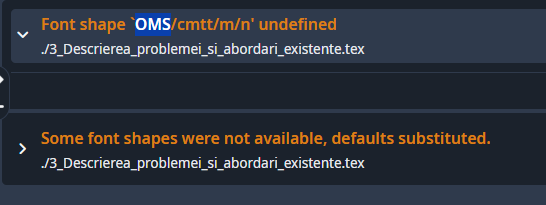
\includegraphics[width=0.8\textwidth]{figs/EroareLatex.png}
    \caption{Exemplu de avertisment de compilare semnalat de Overleaf, pentru care a fost solicitată asistență la depanare.}
    \label{fig:eroare_latex_claude}
\end{figure}

\textbf{Generarea figurilor de tip grid} din Capitolul 4, cu exemple din setul de date procesat (imaginea originală alături de regiunea de interes extrasă corespunzătoare), a fost realizată prin furnizarea imaginilor individuale, în mai multe runde succesive, pe măsură ce grid-ul era completat, și solicitarea compunerii acestora într-o singură imagine. De exemplu, a fost folosit promptul: \textit{"îți mai dau câteva poze cu raci, poți să le pui pe toate într-o singură imagine, tip grid?"}. Figura rezultată a fost verificată vizual, pentru a confirma corectitudinea asocierii dintre fiecare imagine originală și crop-ul corespunzător, înainte de a fi integrată în Capitolul 4,  Figura~\ref{fig:crop_torrentium} și respectiv Figura~\ref{fig:crop_bihariensis}.

\textbf{Identificarea de surse bibliografice suplimentare}, relevante pentru cercetarea prezentată în Capitolul 3, a completat căutarea proprie a autorului cu lucrări conexe și cu surse alternative de acces pentru articole găsite independent, dar inaccesibile prin metodele uzuale de căutare. De exemplu, pentru clarificarea dimensiunii reale de intrare a arhitecturii AlexNet a fost folosit promptul: \textit{"lucrarea originală a lui Krizhevsky zice 224x224 dar cifrele nu se leagă, poți să verifici și să-mi găsești o sursă care explică de ce e de fapt 227x227?"}, care a condus la identificarea implementării de referință \url{https://github.com/dansuh17/alexnet-pytorch} \cite{suh2018alexnet}. Pentru fiecare temă sau articol căutat, au fost solicitate lucrări similare sau linkuri alternative către sursa respectivă. Toate sursele și linkurile propuse au fost verificate manual, prin accesare directă, pentru a confirma existența și relevanța acestora, înainte ca acestea să fie citate în lucrare.

\end{document}